%---------------------------------------------------------------------
\begin{frame}{}

    \begin{center}
        \Large \textcolor{maroon}{Some microeconomics review}
        \end{center}
\end{frame}
%---------------------------------------------------------------------
\begin{frame}{Budget constraint}

    Small economy:
    \begin{itemize}
        \item Two goods $x_1$ and $x_2$
        \item Prices $p_1$ and $p_2$ respectively
        \item Total income available to consumer: $m$
    \end{itemize} 
    \vspace{3mm}

    $\implies$ \newbold{Budget constraint}:

    \begin{equation*}
        \underbrace{p_{1} x_{1}}_{\text{Amount spent on Good 1}}
        +
        \underbrace{p_{2} x_{2}}_{\text{Amount spent on Good 2}}
        = \underbrace{m}_{\text{Income}}
    \end{equation*}


\end{frame}
%---------------------------------------------------------------------
\begin{frame}{Budget constraint}

    \begin{minipage}[c]{0.55\textwidth}
        \hspace{7mm}
        \vspace{5mm}
        \begin{tikzpicture}[scale=1.3]
            
            % Axes
            \draw[->] (0,0) -- (6,0) node[right] {$x_1$};
            \draw[->] (0,0) -- (0,4) node[above] {$x_2$};
        
        \end{tikzpicture}
    \end{minipage}
    \hfill
    \begin{minipage}[c]{0.40\textwidth}
        \vspace{-45mm}
        \begin{equation*}
            p_{1} x_{1}
            +
            p_{2} x_{2}
            = m
        \end{equation*}
    \end{minipage}
 
 \end{frame}
 %---------------------------------------------------------------------
 \begin{frame}{Budget constraint}

    \begin{minipage}[c]{0.55\textwidth}
            \begin{tikzpicture}[scale=1.3]
                
                    % Axes
                    \draw[->] (0,0) -- (6,0) node[right] {$x_1$};
                    \draw[->] (0,0) -- (0,4) node[above] {$x_2$};
                
                    % Intercepts (generic labels)
                    \node at (5.5,-0.3) {$\frac{m}{p_1}$};
                    \node at (-0.6,3.5) {$\frac{m}{p_2}$};
                
                    % Budget line
                    \draw[thick, red] (0,3.5) -- (5.5,0);
                
            \end{tikzpicture}
            
    \end{minipage}
    \hfill
    \begin{minipage}[c]{0.40\textwidth}
        \vspace{-35mm}
        \begin{align*}
            &p_{1} x_{1}
            +
            p_{2} x_{2}
            = m \\
            \Leftrightarrow \text{ } &p_2 x_2 = m - p_1 x_1 \\
            \Leftrightarrow \text{ } &x_2 = \frac{m}{p_2} - \frac{p_1}{p_2} x_1
        \end{align*}
    \end{minipage}
 
 \end{frame}
 %---------------------------------------------------------------------
 \begin{frame}{Budget constraint}

    \begin{minipage}[c]{0.55\textwidth}
        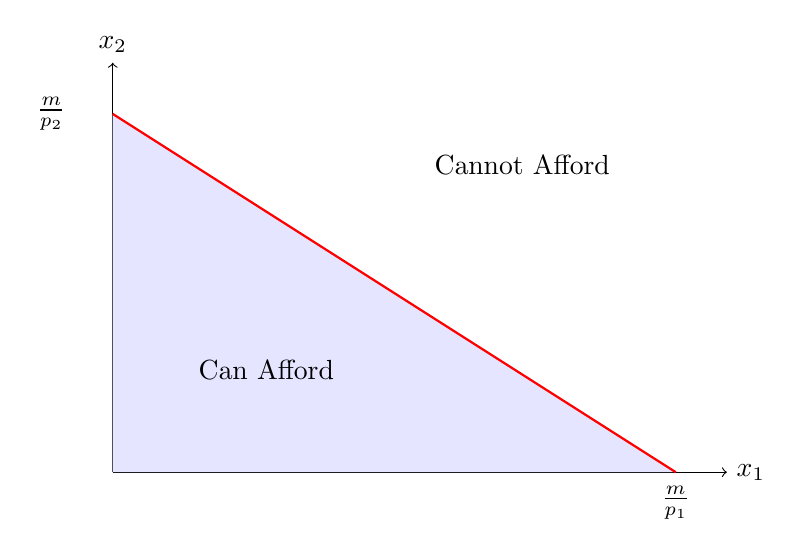
\begin{tikzpicture}[scale=1.3]
        
            % Axes
            \draw[->] (0,0) -- (6,0) node[right] {$x_1$};
            \draw[->] (0,0) -- (0,4) node[above] {$x_2$};
        
            % Intercepts
            \node at (5.5,-0.3) {$\frac{m}{p_1}$};
            \node at (-0.6,3.5) {$\frac{m}{p_2}$};
        
            % Shaded affordable region
            \fill[blue!10] (0,0) -- (0,3.5) -- (5.5,0) -- cycle;
        
            % Budget line (red)
            \draw[thick, red] (0,3.5) -- (5.5,0);
        
            % Labels
            \node at (1.5,1) {Can Afford};
            \node at (4,3) {Cannot Afford};
        
        \end{tikzpicture}
            
    \end{minipage}
    \hfill
    \begin{minipage}[c]{0.40\textwidth}
        \vspace{-35mm}
        \begin{align*}
            &p_{1} x_{1}
            +
            p_{2} x_{2}
            = m \\
            \Leftrightarrow \text{ } &p_2 x_2 = m - p_1 x_1 \\
            \Leftrightarrow \text{ } &x_2 = \frac{m}{p_2} - \frac{p_1}{p_2} x_1
        \end{align*}
    \end{minipage}
 
 \end{frame}
 %---------------------------------------------------------------------
 \begin{frame}{Price change}

    \begin{minipage}[c]{0.55\textwidth}
        \begin{tikzpicture}[scale=1.3]

            % Axes
            \draw[->] (0,0) -- (6,0) node[right] {$x_1$};
            \draw[->] (0,0) -- (0,4) node[above] {$x_2$};
        
            % Old intercepts (before price increase)
            \node at (5.5,-0.3) {$\frac{m}{p_1}$};
            \node at (-0.6,3.3) {$\frac{m}{p_2}$};
        
            % New x1 intercept (after price increase)
            \node at (3.3,-0.3) {$\frac{m}{p_1^*}$};
        
            % Old budget line (before p1 increases)
            \draw[thick, red] (0,3.3) -- (5.5,0);
        
            % New budget line (steeper, after p1 increases)
            \draw[thick, red!60!black, dashed] (0,3.3) -- (3.3,0);

            % Arrow from old intercept to new intercept
            \draw[->, thick, red!60!black] (5,0.15) -- (3.3,0.15);

        
        \end{tikzpicture}
            
    \end{minipage}
    \hfill
    \begin{minipage}[c]{0.40\textwidth}
        \vspace{-45mm}
        Assume $p_1$ \textcolor{red!60!black}{increases}, $p_2$ remains the same:
        \begin{align*}
            &x_2 = \frac{m}{p_2} - \frac{\textcolor{red!60!black}{p_1^*}}{p_2} x_1
        \end{align*}
    \end{minipage}
 
 \end{frame}
 %---------------------------------------------------------------------
 \begin{frame}{Income change}

    \begin{minipage}[c]{0.55\textwidth}
        \only<1>{
            \begin{tikzpicture}[scale=1.25]
    
                % Axes
                \draw[->] (0,0) -- (8,0) node[right] {$x_1$};
                \draw[->] (0,0) -- (0,5) node[above] {$x_2$};
            
                % Intercepts (generic labels)
                \node at (5.5,-0.3) {$\frac{m}{p_1}$};
                \node at (-0.6,3.5) {$\frac{m}{p_2}$};
            
               
                % Original budget line (red)
                \draw[thick, red] (0,3.5) -- (5.5,0);
            
            \end{tikzpicture}
        }

        \only<2>{
            \hspace{-2mm}
        \begin{tikzpicture}[scale=1.25]
    
            % Axes
            \draw[->] (0,0) -- (8,0) node[right] {$x_1$};
            \draw[->] (0,0) -- (0,5) node[above] {$x_2$};
        
            % Intercepts (generic labels)
            \node at (5.5,-0.3) {$\frac{m}{p_1}$};
            \node at (-0.6,3.5) {$\frac{m}{p_2}$};
        
            % Shifted intercept labels
            \node at (-0.6,4.5) {$\frac{m^*}{p_2}$};
            \node at (7.1,-0.3) {$\frac{m^*}{p_1}$};
        
            % Original budget line (red)
            \draw[thick, red] (0,3.5) -- (5.5,0);
        
            % Upward-translated budget line (blue, parallel)
            \draw[thick, blue!60!black] (0,4.5) -- (7.07,0);

            % Arrow showing upward translation
            \draw[->, thick, blue!60!black] (1.2,3) -- (1.2,3.5);
        
        \end{tikzpicture}
        }
            
    \end{minipage}
    \hfill
    \begin{minipage}[c]{0.40\textwidth}
        \vspace{-45mm}
        Assume $m$ \textcolor{blue!60!black}{increases}:
        \begin{align*}
            &x_2 = \frac{\textcolor{blue!60!black}{m^*}}{p_2} - \frac{p_1}{p_2} x_1
        \end{align*}
    \end{minipage}
 
 \end{frame}
%---------------------------------------------------------------------
% Tikz was difficult to tailor to my needs
% \begin{frame}{Preferences: indifference curve}

%     \begin{minipage}[c]{0.55\textwidth}
%         \begin{tikzpicture}[scale=1.3]
%             % Axes (not rotated)
%             \draw[->] (0,0) -- (6,0) node[right] {$x_1$};
%             \draw[->] (0,0) -- (0,5) node[above] {$x_2$};
        
%             % Rotated curve group
%             \begin{scope}[rotate=-15, shift={(-0.5,0)}]
        
%                 % Decreasing convex curve
%                 \draw[thick, blue!30!black]
%                     plot [smooth] coordinates {
%                         (0.6, 4.17)
%                         (1.0, 3.50)
%                         (1.5, 3.17)
%                         (2.0, 3.00)
%                         (3.0, 2.83)
%                         (4.0, 2.75)
%                         (5.0, 2.70)
%                     };
        
%                 % Two points
%                 \fill[gray] (1.0,3.50) circle (2.3pt);
%                 \fill[gray] (3.0,2.83) circle (2.3pt);
        
%                 % Tangent line between the points (straight decreasing line)
%                 \draw[dashed, thick, red]
%                     (1.0,3.50) -- (3.0,2.83);
        
%             \end{scope}
%         \end{tikzpicture}
%     \end{minipage}
%     \hfill
%     \begin{minipage}[c]{0.40\textwidth}
%         \vspace{-45mm}
%         \begin{equation*}
%             U(x_1, x_2) = \bar{U}
%         \end{equation*}
%     \end{minipage}
 
%  \end{frame}
% %---------------------------------------------------------------------
\begin{frame}{Preferences: indifference curve}

    \begin{minipage}[c]{0.55\textwidth}
    \begin{center}
        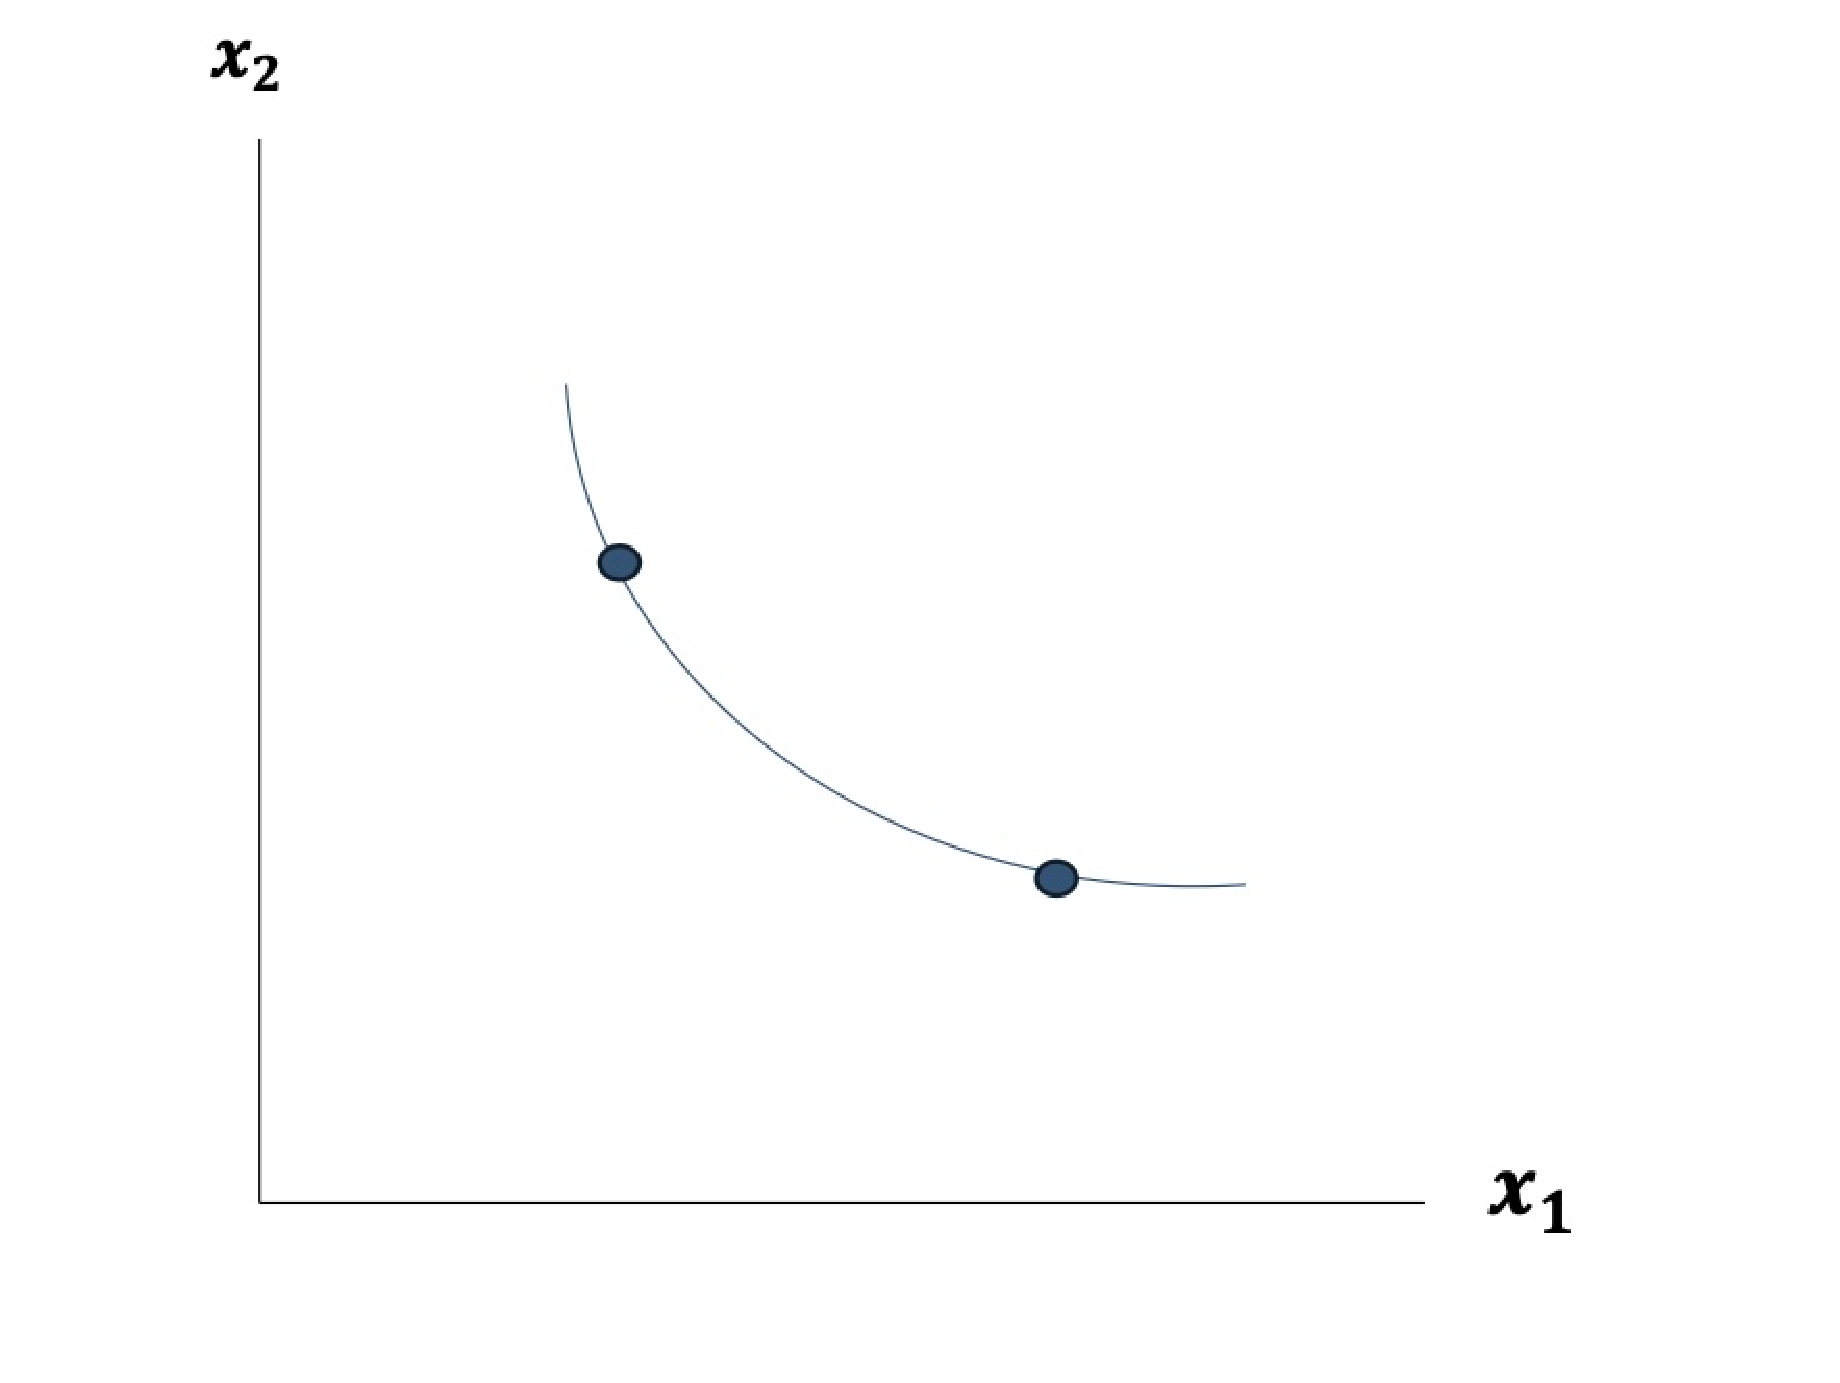
\includegraphics[width=1.1\textwidth]{input/indifference_curve_BC_1.pdf}
    \end{center}
    \end{minipage}
    \hfill
    \begin{minipage}[c]{0.40\textwidth}
        \begin{equation*}
            U(x_1, x_2) = \bar{U}
        \end{equation*}
        \vspace{45mm}

    \end{minipage}
 
 \end{frame}
%---------------------------------------------------------------------
\begin{frame}{Preferences: indifference curve}

    \begin{minipage}[c]{0.55\textwidth}
        \hspace{-10mm}
        \vspace{-8mm}
    \begin{center}
        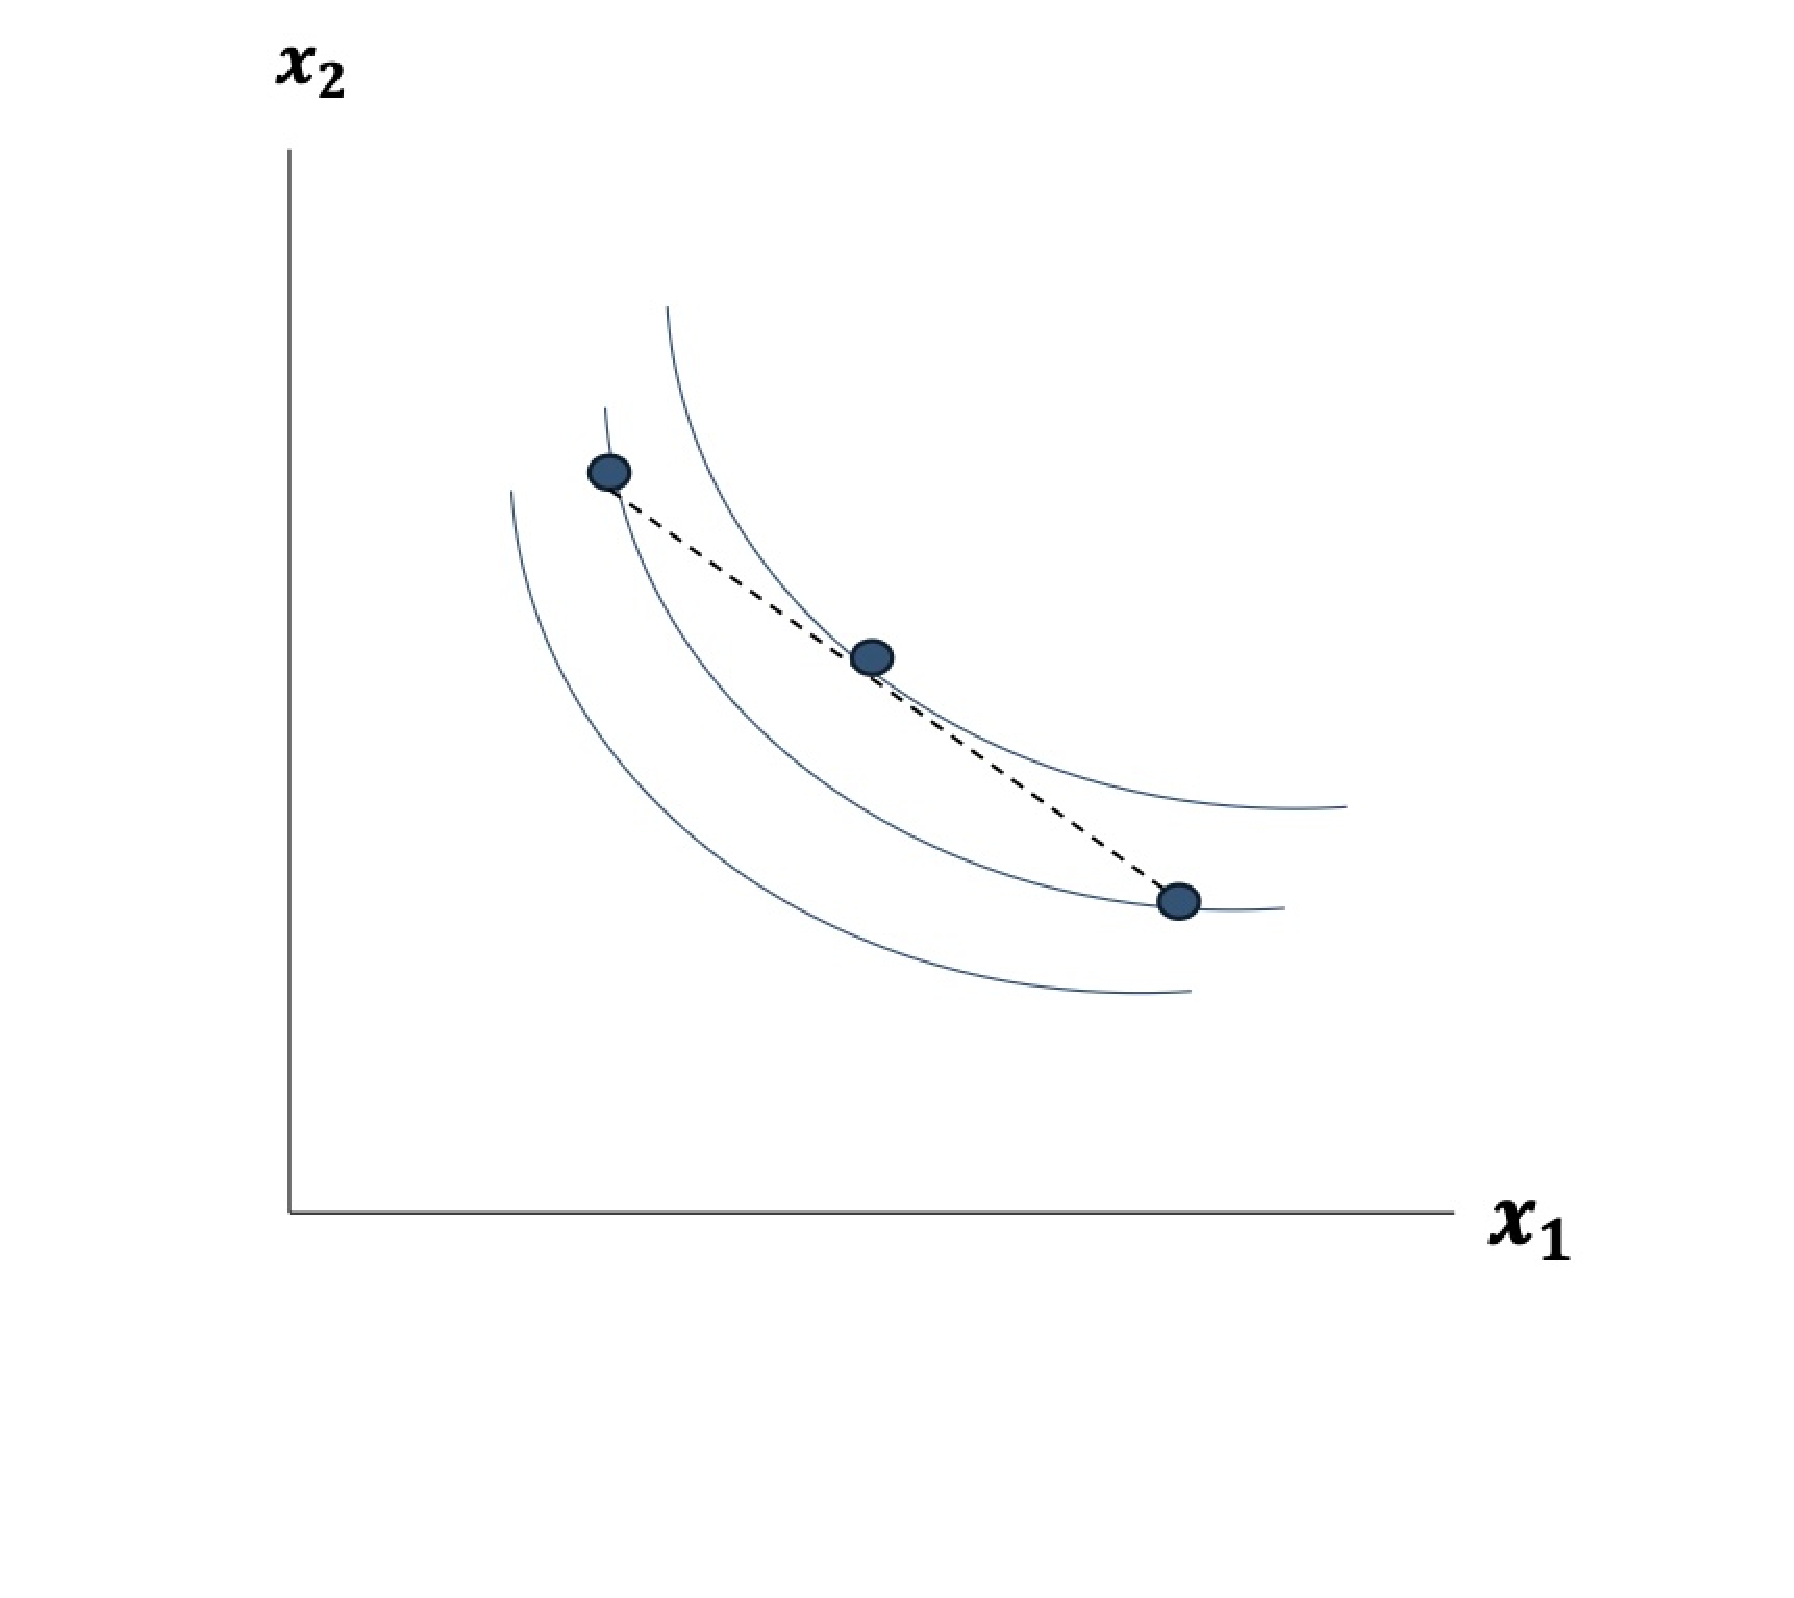
\includegraphics[width=1.1\textwidth]{input/indifference_curve_BC_2.pdf}
    \end{center}
    \end{minipage}
    \hfill
    \begin{minipage}[c]{0.40\textwidth}
        \begin{equation*}
            U(x_1, x_2) = \bar{U}
        \end{equation*}
        \vspace{5mm}
        \\
        Average better than extremes
        \vspace{40mm}

    \end{minipage}
 
 \end{frame}
%---------------------------------------------------------------------
\begin{frame}{Demand}

    \begin{minipage}[c]{0.55\textwidth}
    \begin{center}
        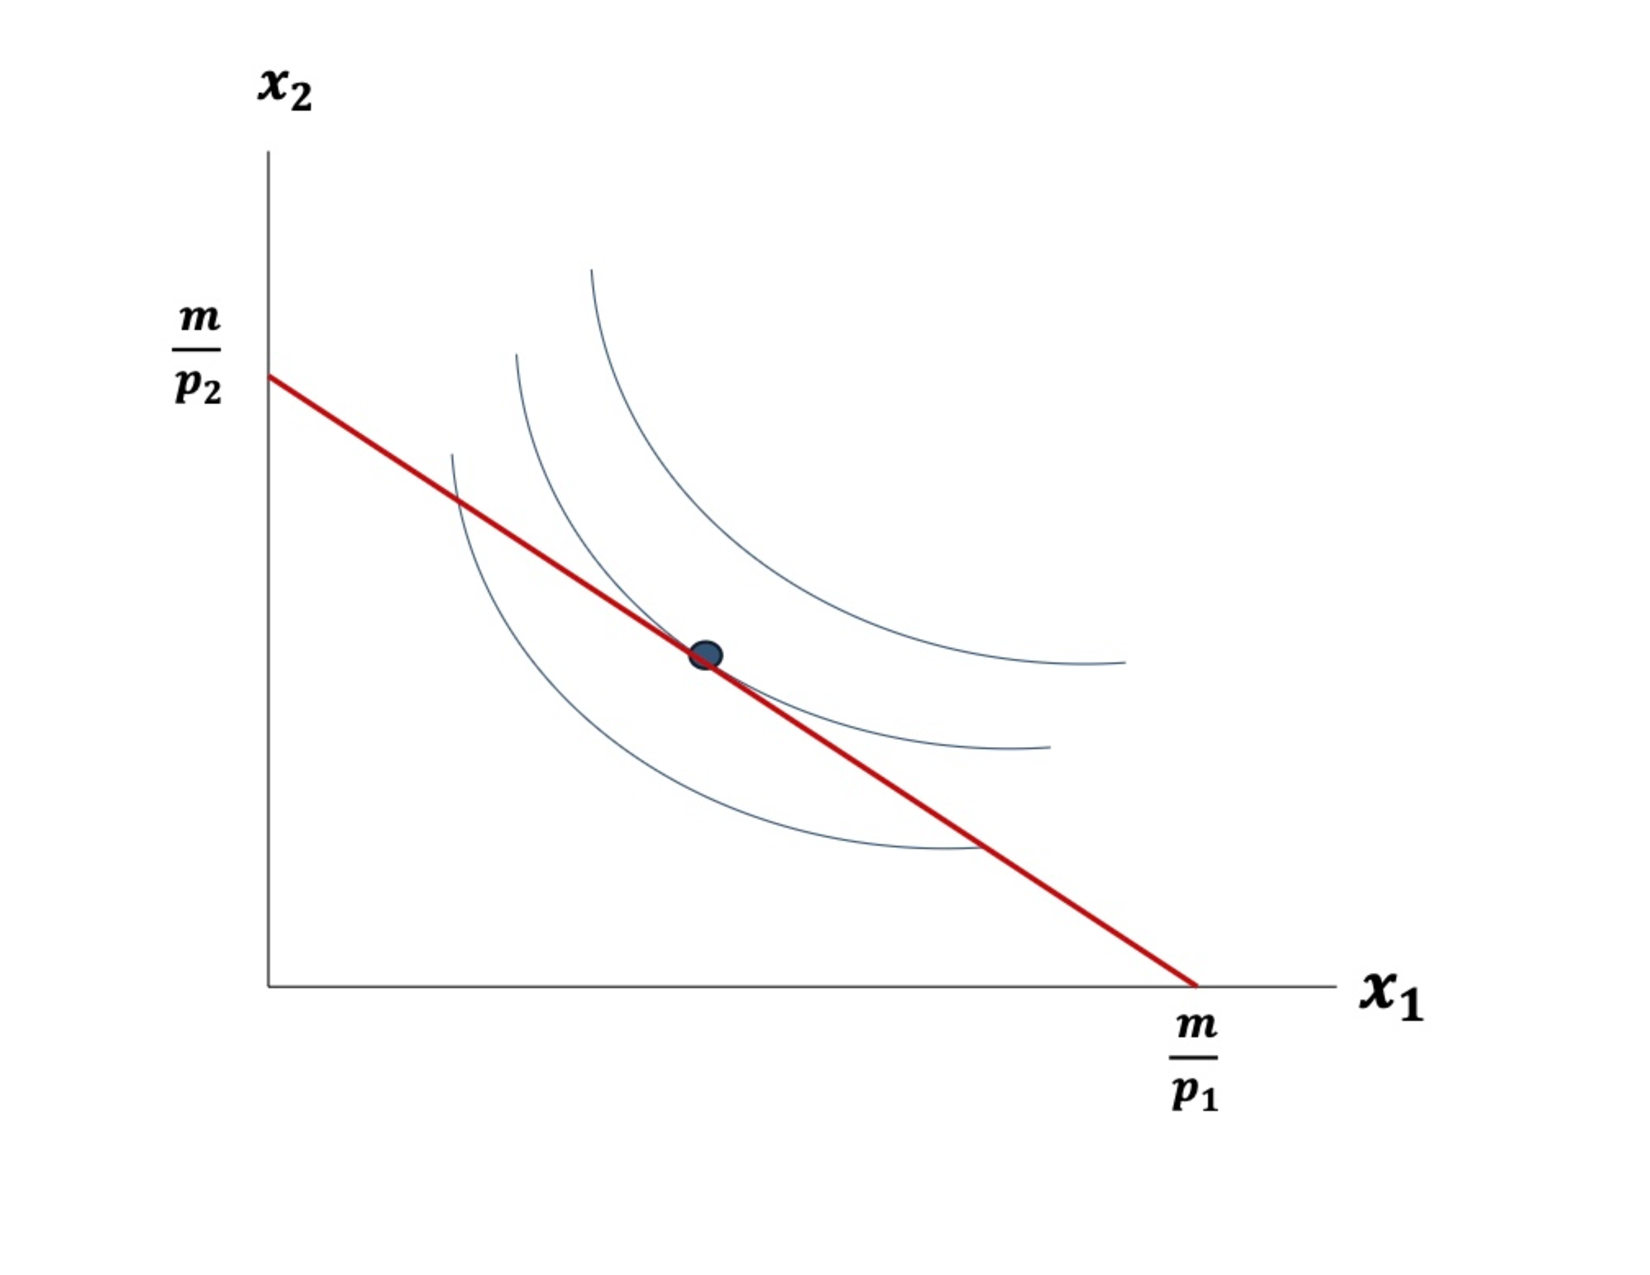
\includegraphics[width=1.1\textwidth]{input/indifference_curve_BC_3.pdf}
    \end{center}
    \end{minipage}
    \hfill
    \begin{minipage}[c]{0.40\textwidth}
        \vspace{-45mm}
        \begin{align*}
            &\max_{x_1,x_2} U(x_1, x_2)\\
            \text{s.t.   } &p_1 x_1 + p_2 x_2 = m
        \end{align*}
    \end{minipage}
 
 \end{frame}
%---------------------------------------------------------------------
\begin{frame}{Demand}

    \begin{minipage}[c]{0.55\textwidth}
    \begin{center}
        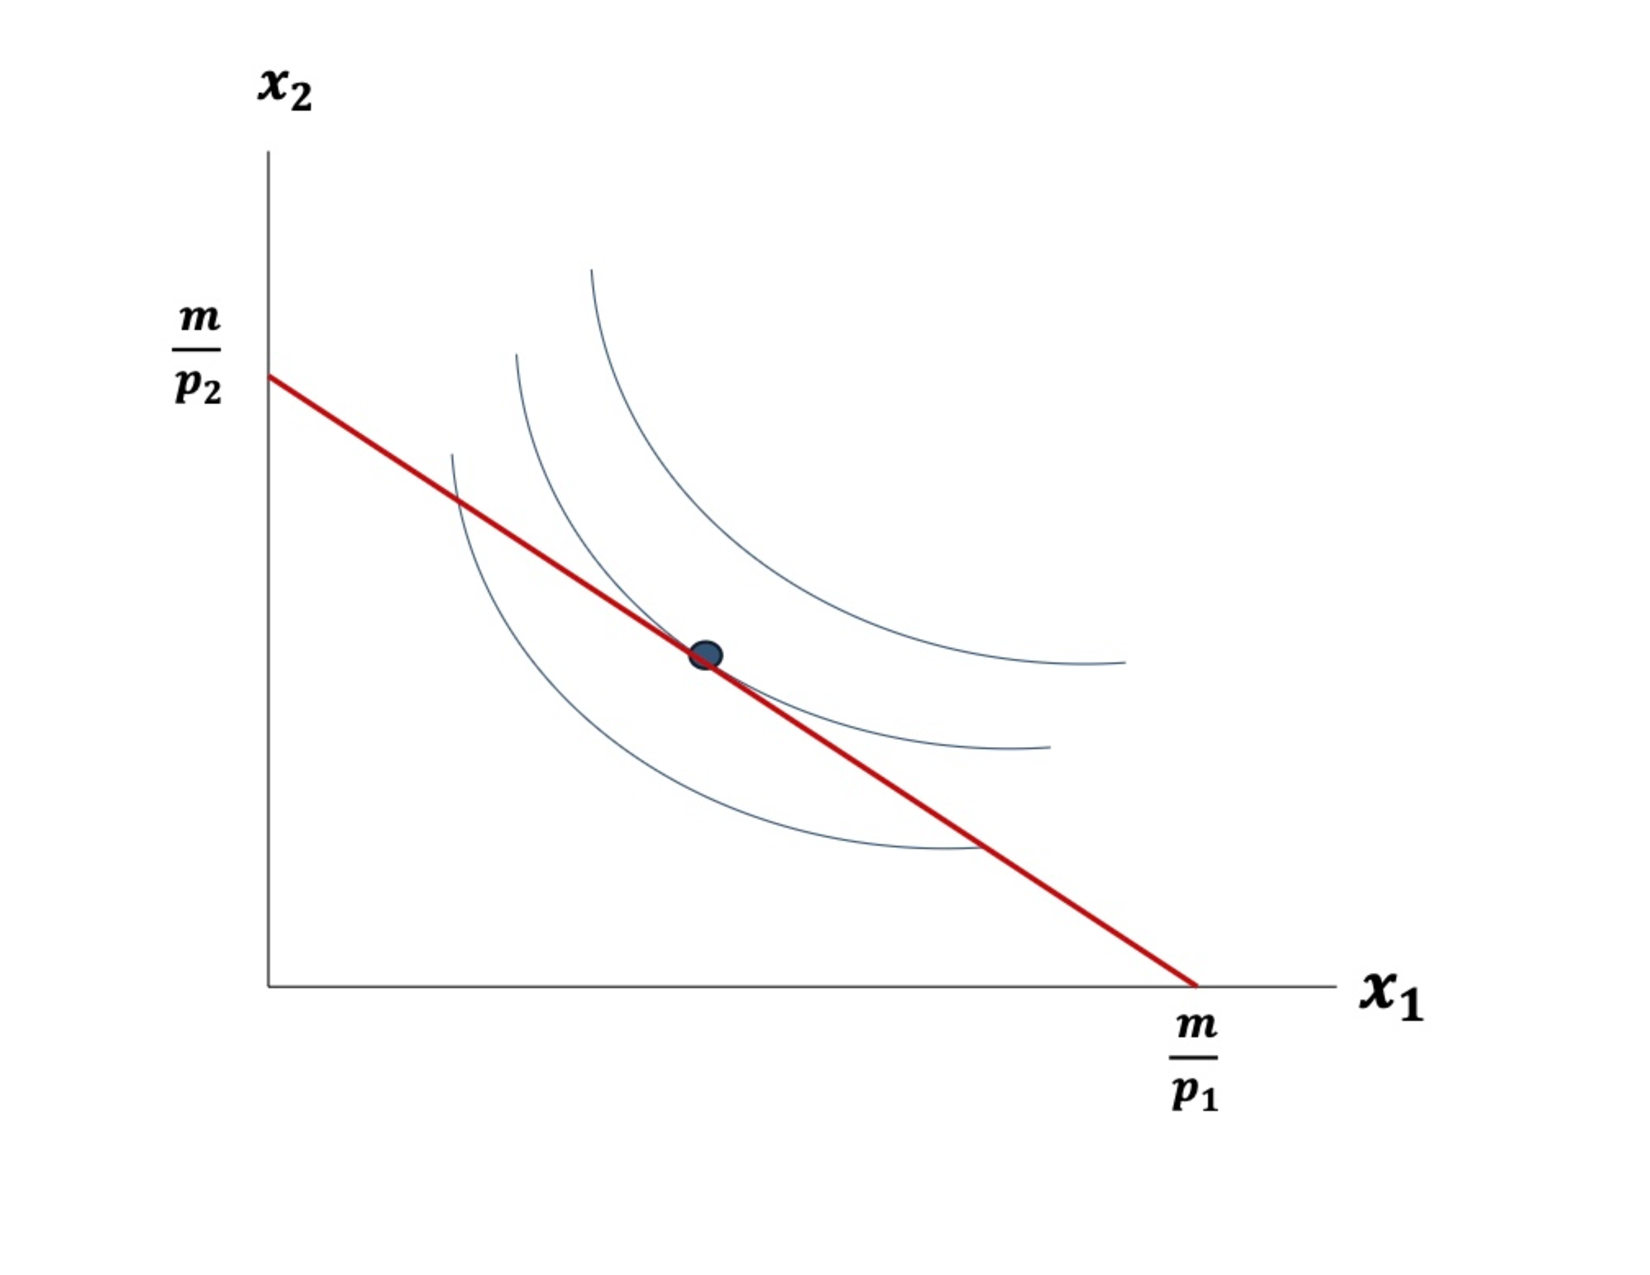
\includegraphics[width=1.1\textwidth]{input/indifference_curve_BC_3.pdf}
    \end{center}
    \end{minipage}
    \hfill
    \begin{minipage}[c]{0.40\textwidth}
        \begin{align*}
            &\max_{x_1,x_2} U(x_1, x_2)\\
            \text{s.t.   } &p_1 x_1 + p_2 x_2 = m
        \end{align*}
        \vspace{3mm}
        \\
        What if price of good 1 \newbold{increases}? $p_1^*$
        \vspace{15mm}
    \end{minipage}
 
 \end{frame}
%---------------------------------------------------------------------
\begin{frame}{Demand}

    \begin{minipage}[c]{0.55\textwidth}
    \begin{center}
        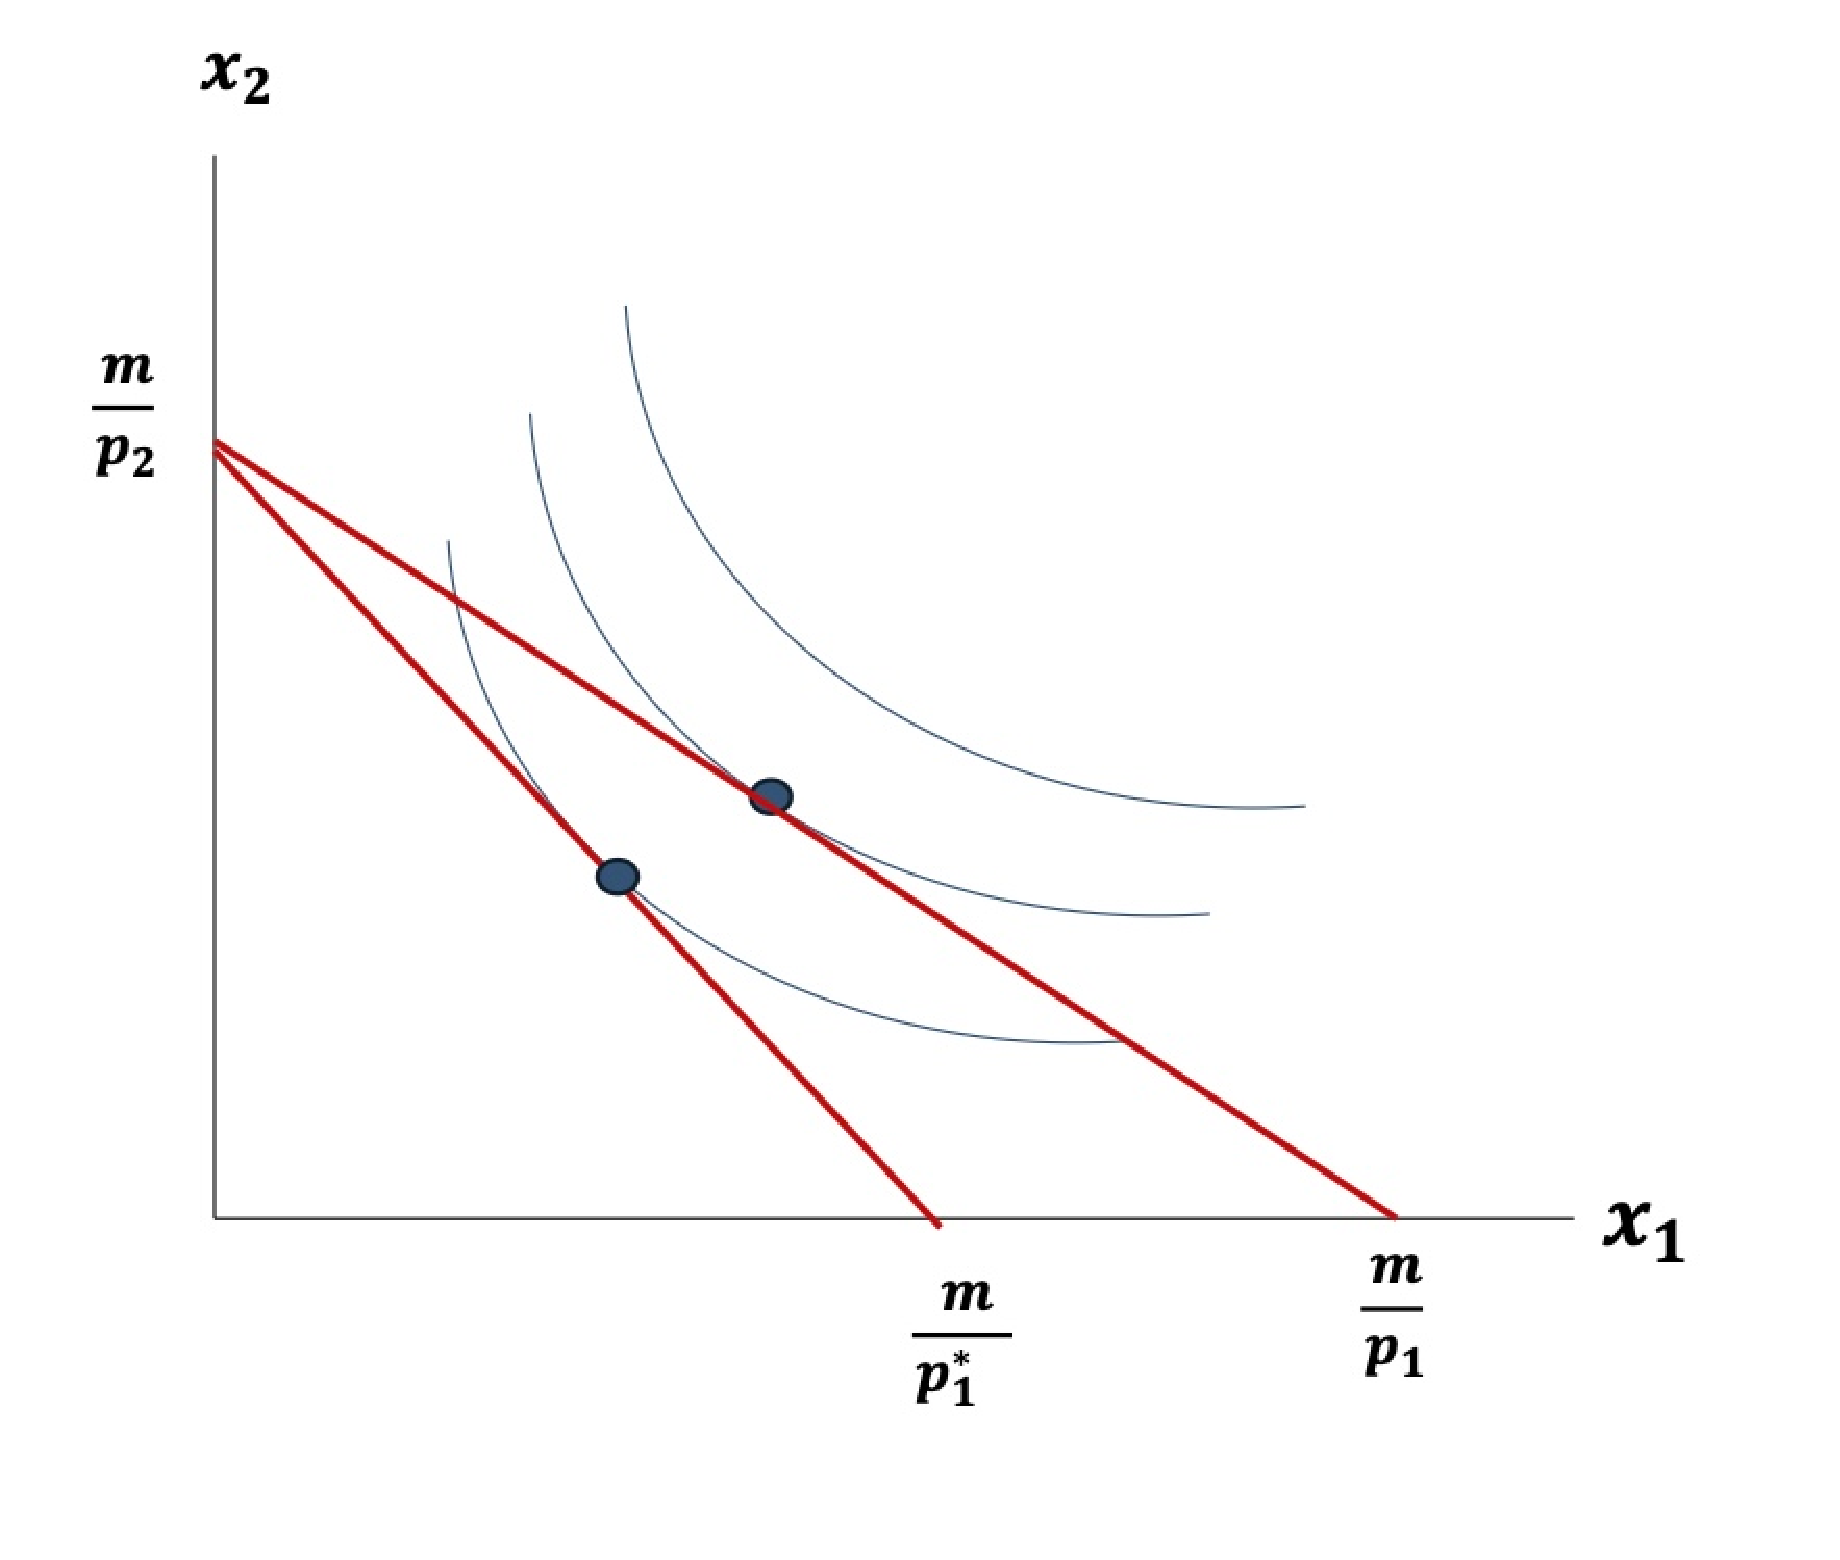
\includegraphics[width=1.1\textwidth]{input/indifference_curve_BC_4.pdf}
    \end{center}
    \end{minipage}
    \hfill
    \begin{minipage}[c]{0.40\textwidth}
        \begin{align*}
            &\max_{x_1,x_2} U(x_1, x_2)\\
            \text{s.t.   } &p_1 x_1 + p_2 x_2 = m
        \end{align*}
        \vspace{3mm}
        \\
        What if price of good 1 \newbold{increases}? $p_1^*$
        \vspace{15mm}
    \end{minipage}
 
 \end{frame}
%---------------------------------------------------------------------
\begin{frame}{Demand}

    \begin{minipage}[c]{0.55\textwidth}
    \begin{center}
        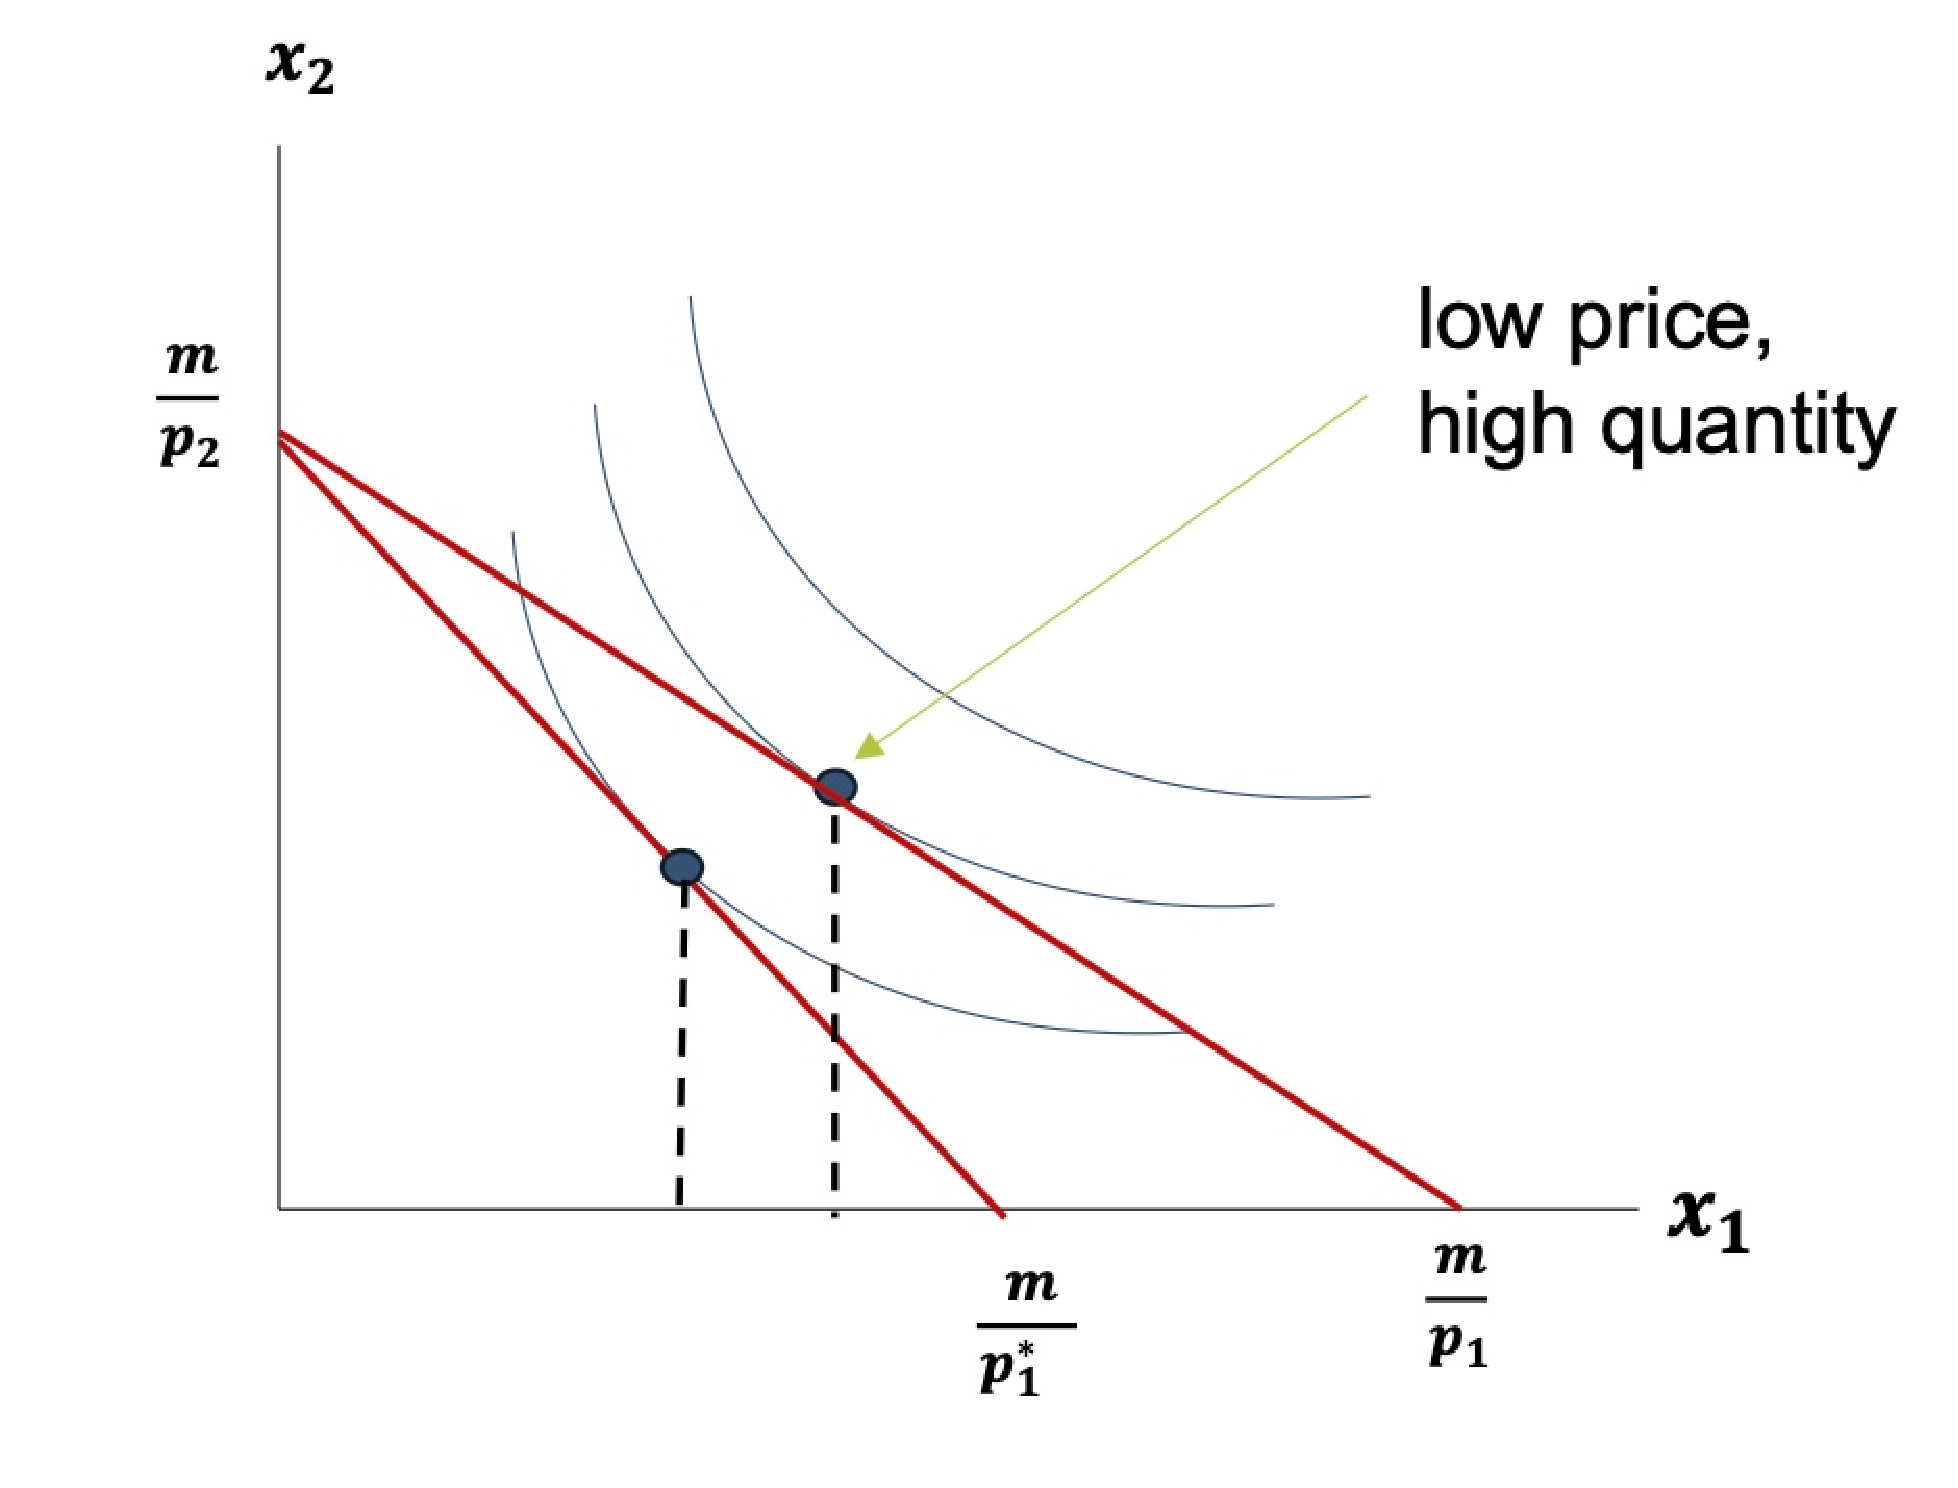
\includegraphics[width=1.1\textwidth]{input/indifference_curve_BC_5.pdf}
    \end{center}
    \end{minipage}
    \hfill
    \begin{minipage}[c]{0.40\textwidth}
    \end{minipage}
 
 \end{frame}
%---------------------------------------------------------------------
\begin{frame}{Demand}

    \begin{minipage}[c]{0.55\textwidth}
    \begin{center}
        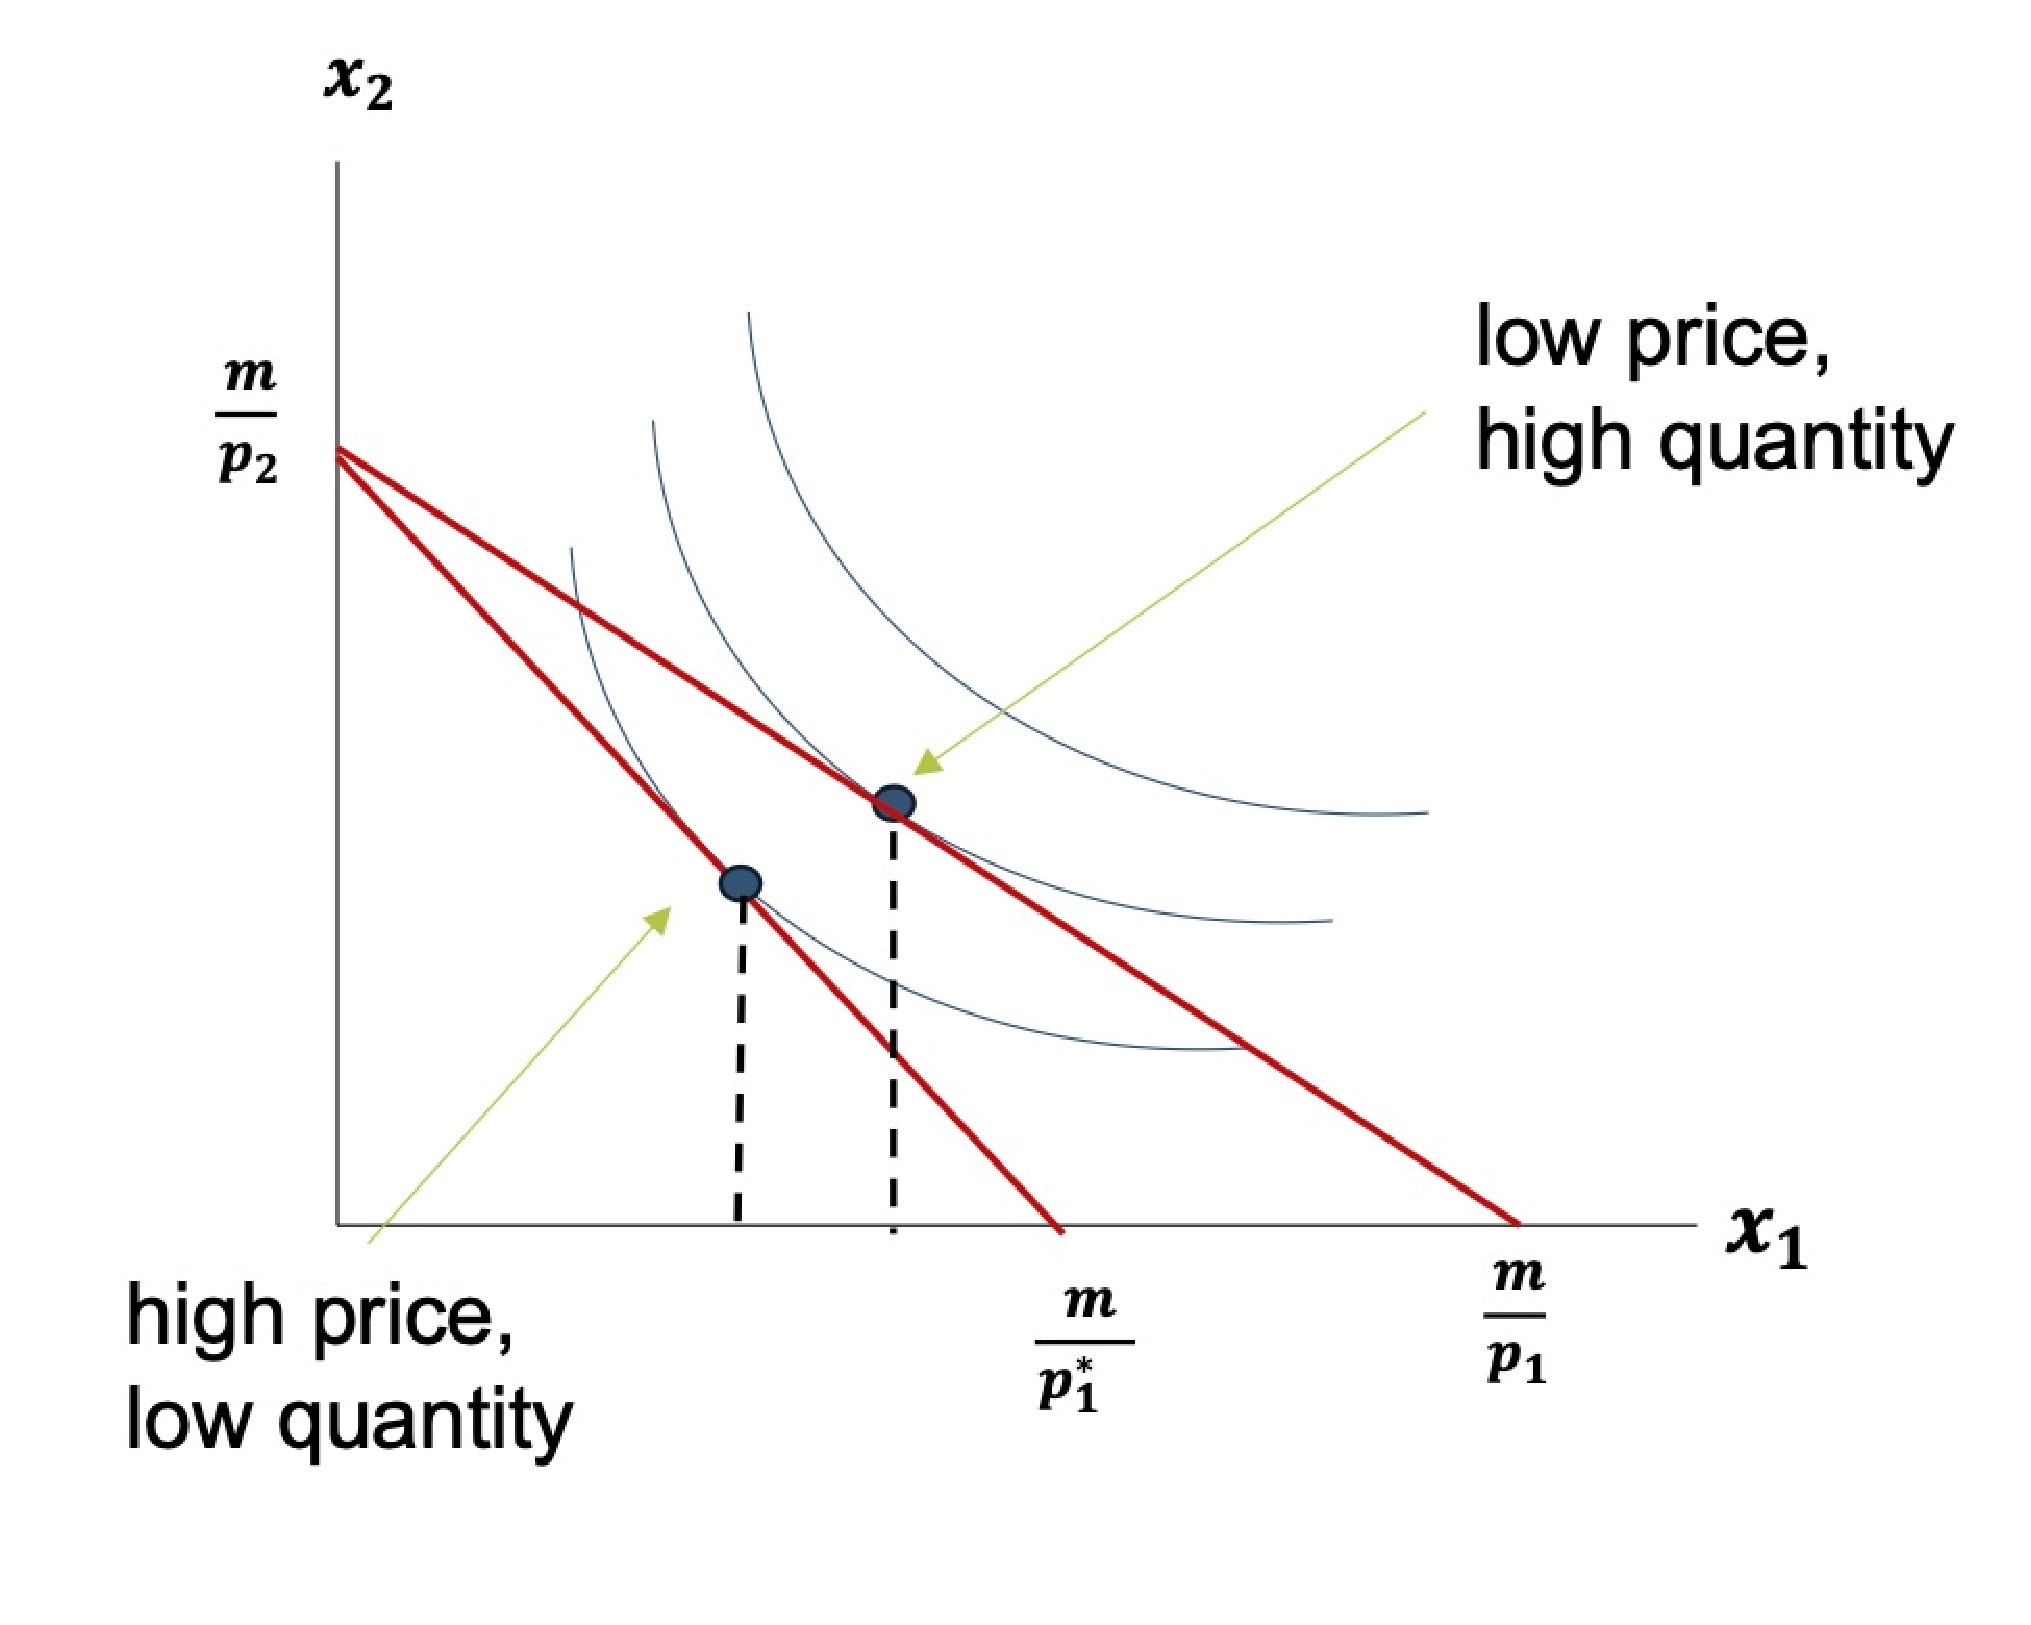
\includegraphics[width=1.15\textwidth]{input/indifference_curve_BC_6.pdf}
    \end{center}
    \end{minipage}
    \hfill
    \begin{minipage}[c]{0.40\textwidth}
    \end{minipage}
 
 \end{frame}
%---------------------------------------------------------------------
\begin{frame}{Demand}

    \begin{center}
        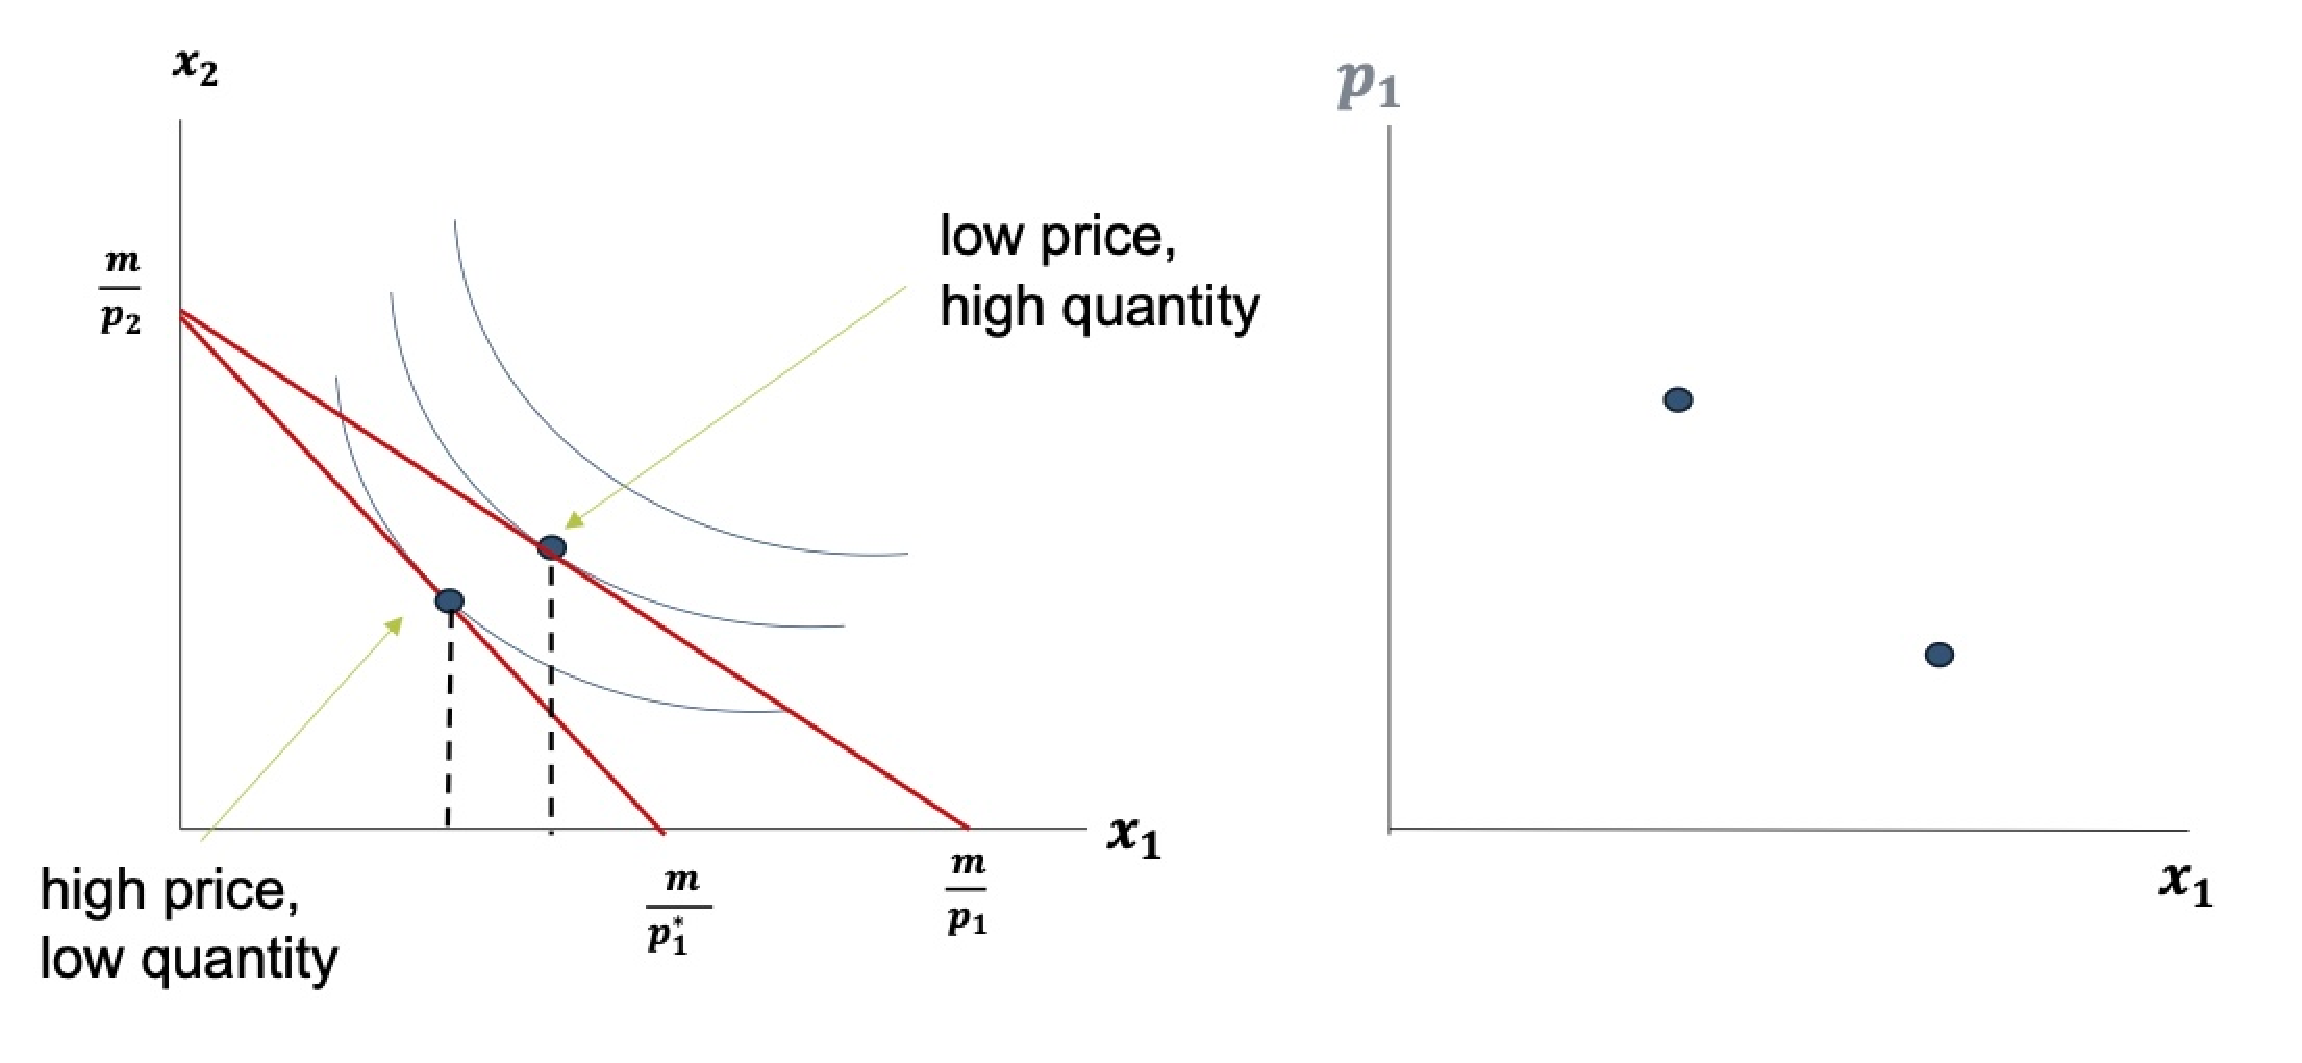
\includegraphics[width=0.95\textwidth]{input/indifference_curve_BC_7.pdf}
    \end{center}
 
 \end{frame}
%---------------------------------------------------------------------
\begin{frame}{Demand}
\begin{center}
    \begin{tikzpicture}[scale=0.9]

        %----- AXES -----
        \draw[thick] (0,0) -- (8,0) node[right, font=\large] {$x_1$};
        \draw[thick] (0,0) -- (0,6) node[above, font=\large] {$p_1$};
    
        %----- EXTENDED BLUE LINE TOUCHING BOTH AXES -----
        \draw[very thin, blue!50!black]
            (0,5.33) -- (7.5,0);
    
        %----- 7 DOTS ON THE BLUE LINE -----
        % Parametric representation of points between (0,5.33) and (7.5,0)
        \foreach \i in {0,...,6} {
            \pgfmathsetmacro{\t}{\i/6}
            \pgfmathsetmacro{\x}{0 + \t*(7.5 - 0)}
            \pgfmathsetmacro{\y}{5.33 + \t*(0 - 5.33)}
    
            \filldraw[
                fill=blue!50!black,
                draw=gray,
                line width=0.4pt
            ] (\x,\y) circle (3pt);
        }
    
    \end{tikzpicture}
\end{center}
 \textcolor{white}{$\implies$ This is the demand for good 1 $p_1(x_1)$.}
 \end{frame}
%---------------------------------------------------------------------
\begin{frame}{Demand}
    \begin{center}
        \begin{tikzpicture}[scale=0.9]

            %----- AXES -----
            \draw[thick] (0,0) -- (8,0) node[right, font=\large] {$x_1$};
            \draw[thick] (0,0) -- (0,6) node[above, font=\large] {$p_1$};
        
            %----- EXTENDED BLUE LINE TOUCHING BOTH AXES -----
            % Line has slope approximately -2/3 and passes near (0.5,5)
            \draw[very thin, blue!50!black]
                (0,5.33) -- (7.5,0);
        
        \end{tikzpicture}
    \end{center}
    $\implies$ This is the \newbold{demand} for good 1 $p_1(x_1)$.
     
\end{frame}
%---------------------------------------------------------------------
\begin{frame}{Increase in demand versus move \textit{along} the demand}
    \begin{minipage}[c]{0.55\textwidth}
        \begin{center}
            \begin{tikzpicture}[scale=0.7]

                %----- AXES -----
                \draw[thick] (0,0) -- (8,0) node[right, font=\large] {$x_1$};
                \draw[thick] (0,0) -- (0,6) node[above, font=\large] {$p_1$};
            
                %----- EXTENDED BLUE LINE TOUCHING BOTH AXES -----
                \draw[very thin, blue!50!black]
                    (0,5.33) -- (7.5,0);
            
                %----- TWO DOTS (upper and lower) -----
                % Upper dot at t = 0.2
                \pgfmathsetmacro{\tU}{0.2}
                \pgfmathsetmacro{\xU}{\tU*7.5}
                \pgfmathsetmacro{\yU}{5.33*(1 - \tU)}
                \filldraw[fill=blue!50!black, draw=gray, line width=0.4pt]
                    (\xU,\yU) circle (3pt);
            
                % Lower dot at t = 0.6
                \pgfmathsetmacro{\tL}{0.6}
                \pgfmathsetmacro{\xL}{\tL*7.5}
                \pgfmathsetmacro{\yL}{5.33*(1 - \tL)}
                \filldraw[fill=blue!50!black, draw=gray, line width=0.4pt]
                    (\xL,\yL) circle (3pt);
            
                %----- SHORTER PARALLEL ARROW ABOVE THE LINE -----
                % Shift upward and shorten horizontally by using t = 0.25 → 0.55
                \pgfmathsetmacro{\tA}{0.25}
                \pgfmathsetmacro{\xA}{\tA*7.5}
                \pgfmathsetmacro{\yA}{5.33*(1 - \tA)}
            
                \pgfmathsetmacro{\tB}{0.55}
                \pgfmathsetmacro{\xB}{\tB*7.5}
                \pgfmathsetmacro{\yB}{5.33*(1 - \tB)}
            
                % Vertical shift upward
                \pgfmathsetmacro{\shift}{0.35}
            
                \draw[->, thick, blue!50!black]
                    (\xA, \yA+\shift) -- (\xB, \yB+\shift);
            
        \end{tikzpicture}  

        (a) Move \textit{along} the demand curve
        \end{center}
        \end{minipage}
        \hfill
        \begin{minipage}[c]{0.40\textwidth}
        \begin{center}
            \begin{tikzpicture}[scale=0.7]

                %----- AXES -----
                \draw[thick] (0,0) -- (8,0) node[right, font=\large] {$x_1$};
                \draw[thick] (0,0) -- (0,6) node[above, font=\large] {$p_1$};
            
                %----- ORIGINAL BLUE LINE -----
                \draw[very thin, blue!50!black]
                    (0,5.33) -- (7.5,0);
            
                %----- PARALLEL SHIFTED LINE (dashed, asymmetric length) -----
                \def\shift{1.2}
            
                \draw[very thin, red!50!black, dashed]
                    (1,   {5.33 - (5.33/7.5)*1   + \shift})
                    --
                    (7.2, {5.33 - (5.33/7.5)*7.2 + \shift});
            
                %----- ARROW BETWEEN THE TWO LINES (LOWERED SLIGHTLY MORE) -----
                \def\xarrow{3.3}
                \def\yorig{5.33 - (5.33/7.5)*3.3}
                \def\yshifted{\yorig + \shift}
            
                % tiny bit lower: -0.35 instead of -0.25
                \pgfmathsetmacro{\ymid}{(\yorig + \yshifted)/2 - 0.35}
            
                \draw[->, thick, red!50!black]
                    (\xarrow, {\ymid})
                    --
                    ({\xarrow + 1}, {\ymid});
            
            \end{tikzpicture}
            (b) Increase in demand
        \end{center}
        \end{minipage}     
\end{frame}
%---------------------------------------------------------------------
\begin{frame}{}

    \begin{center}
        \Large \textcolor{maroon}{Is the demand for healthcare different than other goods?}
        \end{center}
\end{frame}
%---------------------------------------------------------------------
\begin{frame}{What is cost-sharing?}

        \newbold{Cost-sharing}: portion of medical bill that the patient is responsible for paying
        \vspace{5mm}

        Demand slopes \newbold{down}
        \begin{enumerate}
            \item Is this true in healthcare? \only<2>{\newbold{Late 70s: was a debate.}}
            \item If so, to what extent? \only<2-3>{\textit{Elasticity of healthcare demand}}
            \item What does this mean for insurance?
        \end{enumerate}
\end{frame}
%---------------------------------------------------------------------
\begin{frame}{The \newbold{RAND health insurance experiment}}

    \textcolor{gray}{\textit{Back to the late 70s in California...}}
    \begin{center}
    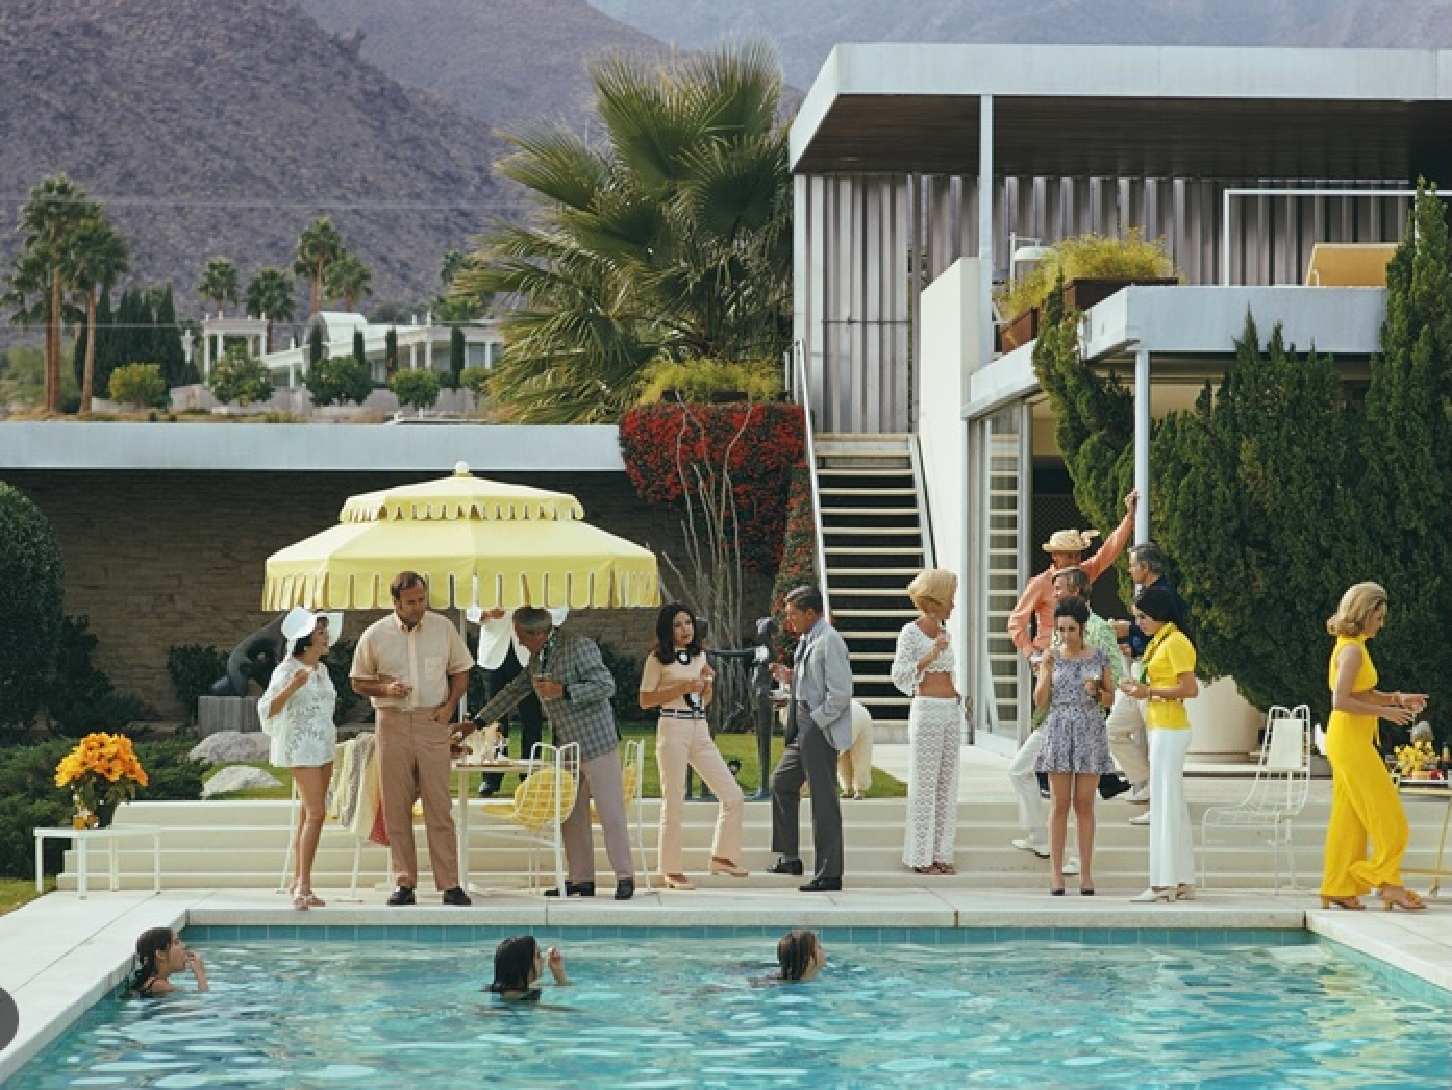
\includegraphics[width=0.5\textwidth]{input/CA_70s.pdf}
    \end{center}

\end{frame}
%---------------------------------------------------------------------
\begin{frame}{Reading: the RAND health insurance experiment}

    \begin{center}
        
\includegraphics[width=0.6\textwidth]{input/RAND_frontarticle.pdf}
    \end{center}
\end{frame}
%---------------------------------------------------------------------
\begin{frame}{The \newbold{RAND health insurance experiment}}

    The \newbold{RAND health insurance experiment}
        \begin{itemize}
            \item Joe Newhouse (PI) at the RAND corporation
            \item 1974-1981: randomize $\approx$ 2,000 families into plans with \newbold{different cost-sharing}
            \item Duration of experiment: 3-5 years
            \item 6 enrollment sites
            \item Outcomes of interest: health spending and health
        \end{itemize}
        \vspace{3mm}
  
        
    A pioneering study
        \begin{itemize}
            \item One of the largest experiments (\$300 million in2011 dollars)
            \item Screening questionnaires
            \item The experiment \textbf{acts as your insurer}
        \end{itemize}

\end{frame}
%---------------------------------------------------------------------
\begin{frame}{The \newbold{RAND health insurance experiment}}

    \begin{center}
        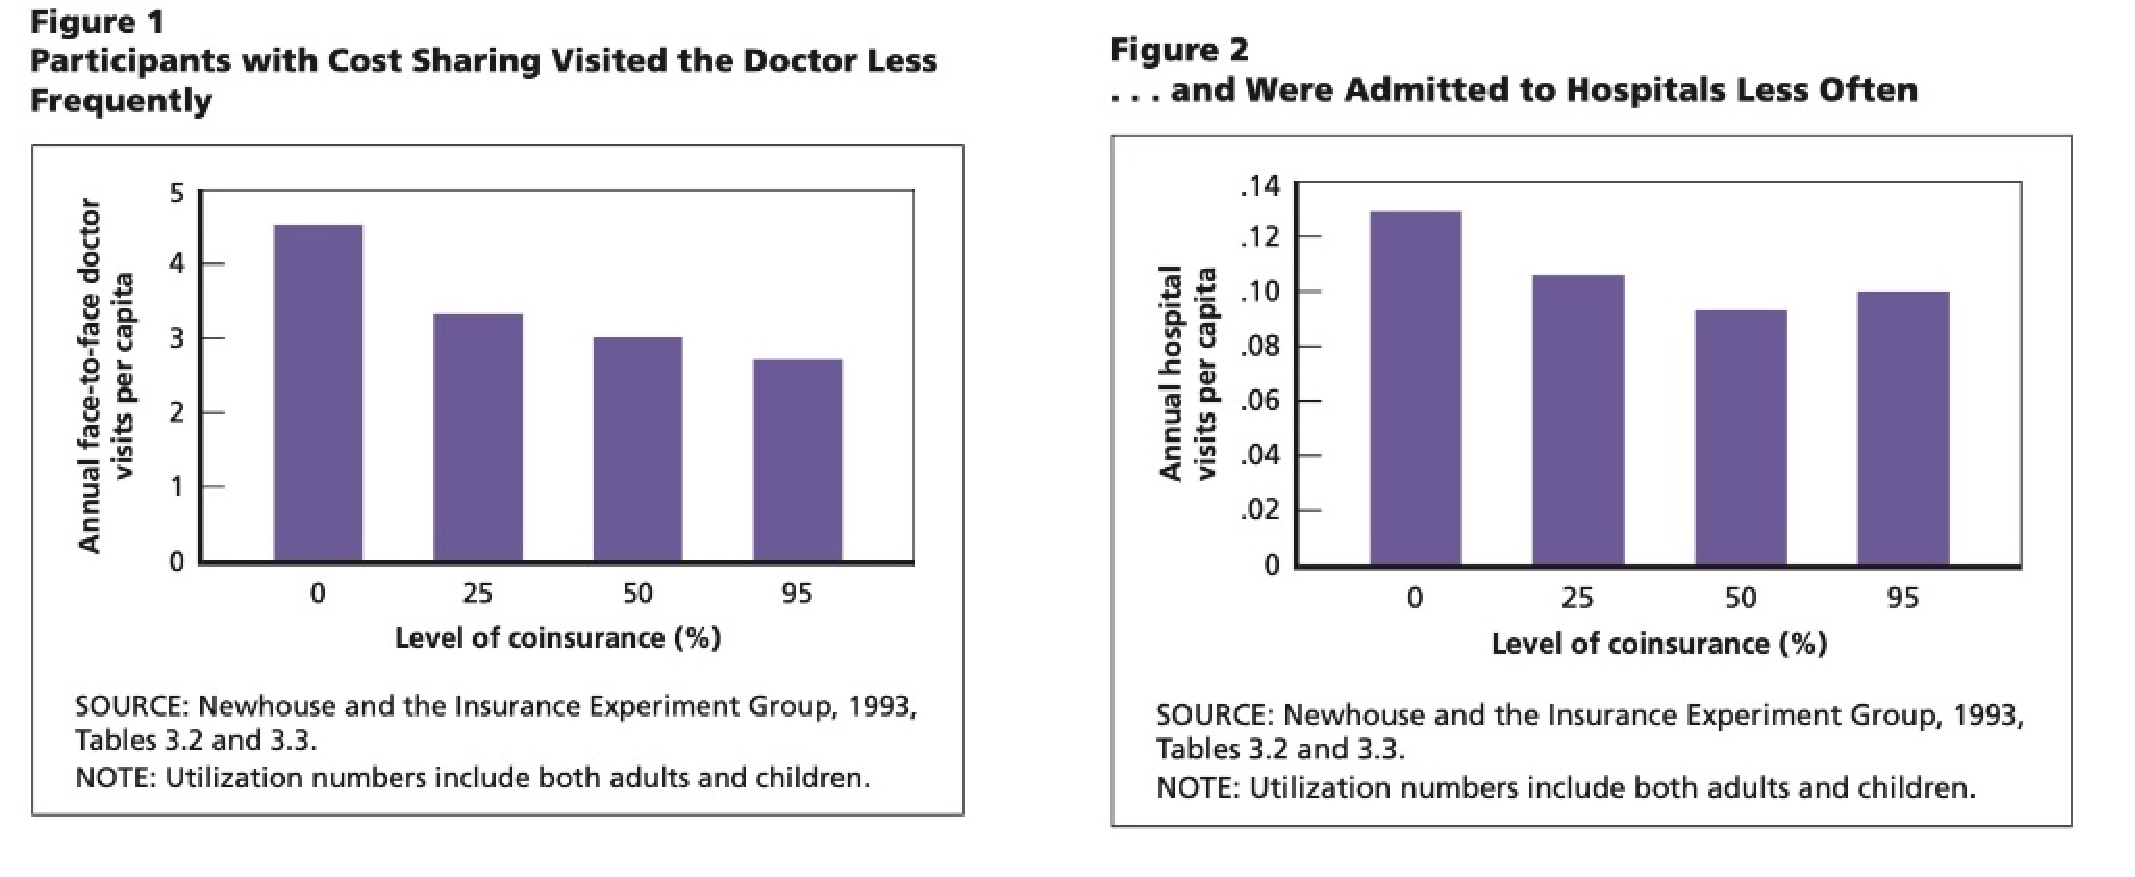
\includegraphics[width=1\textwidth]{input/RAND_fig1and2.pdf}
    \end{center}

\end{frame}
%---------------------------------------------------------------------
\begin{frame}{The \newbold{RAND health insurance experiment}}

    \begin{center}
        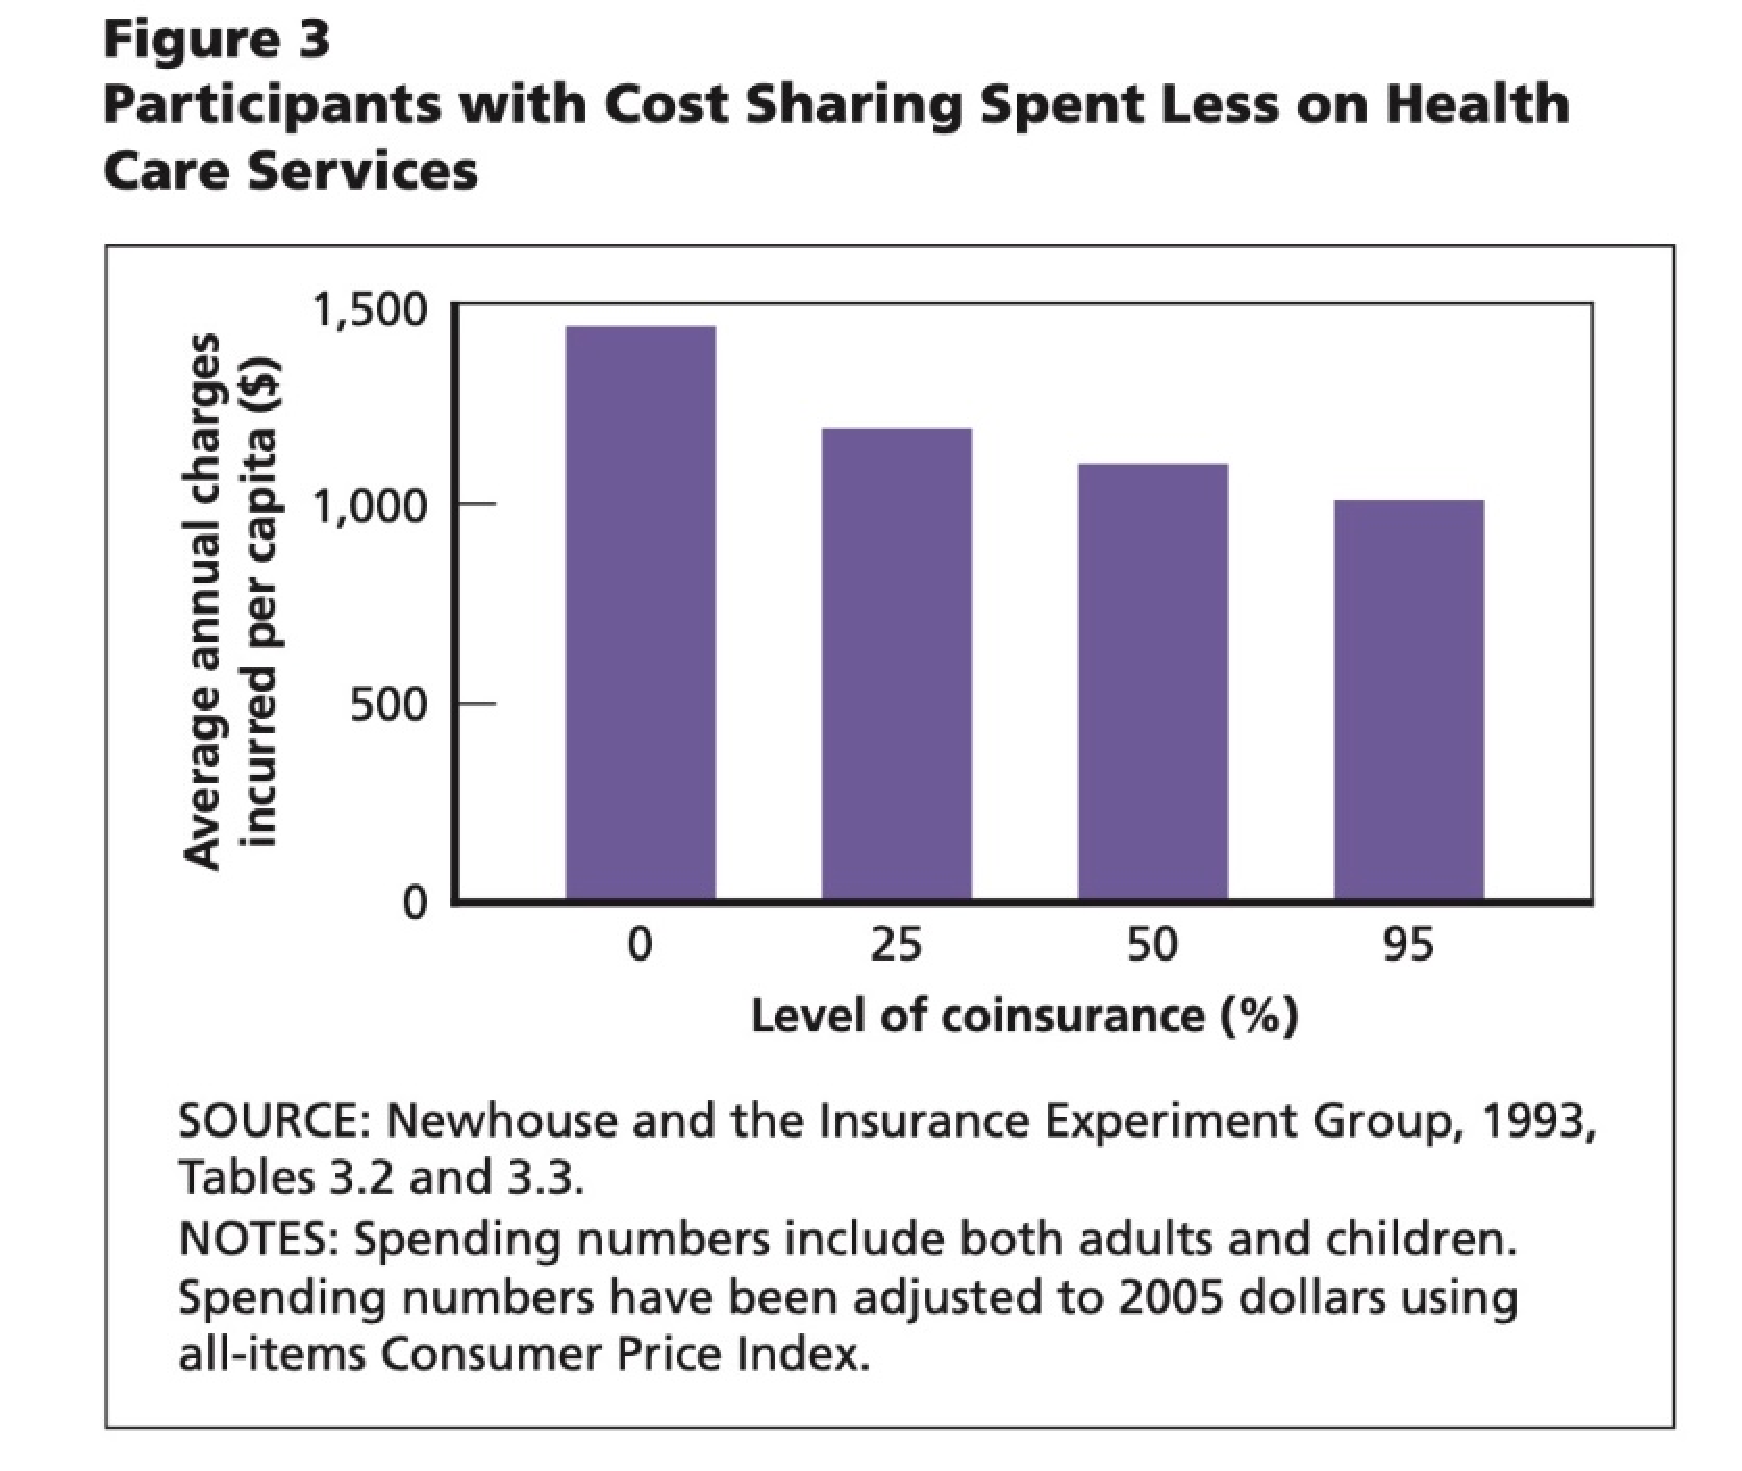
\includegraphics[width=0.6\textwidth]{input/RAND_figure3.pdf}
    \end{center}

\end{frame}
%---------------------------------------------------------------------
\begin{frame}{Which kind of care is consumed less?}

    \only<1>{
    \begin{center}
        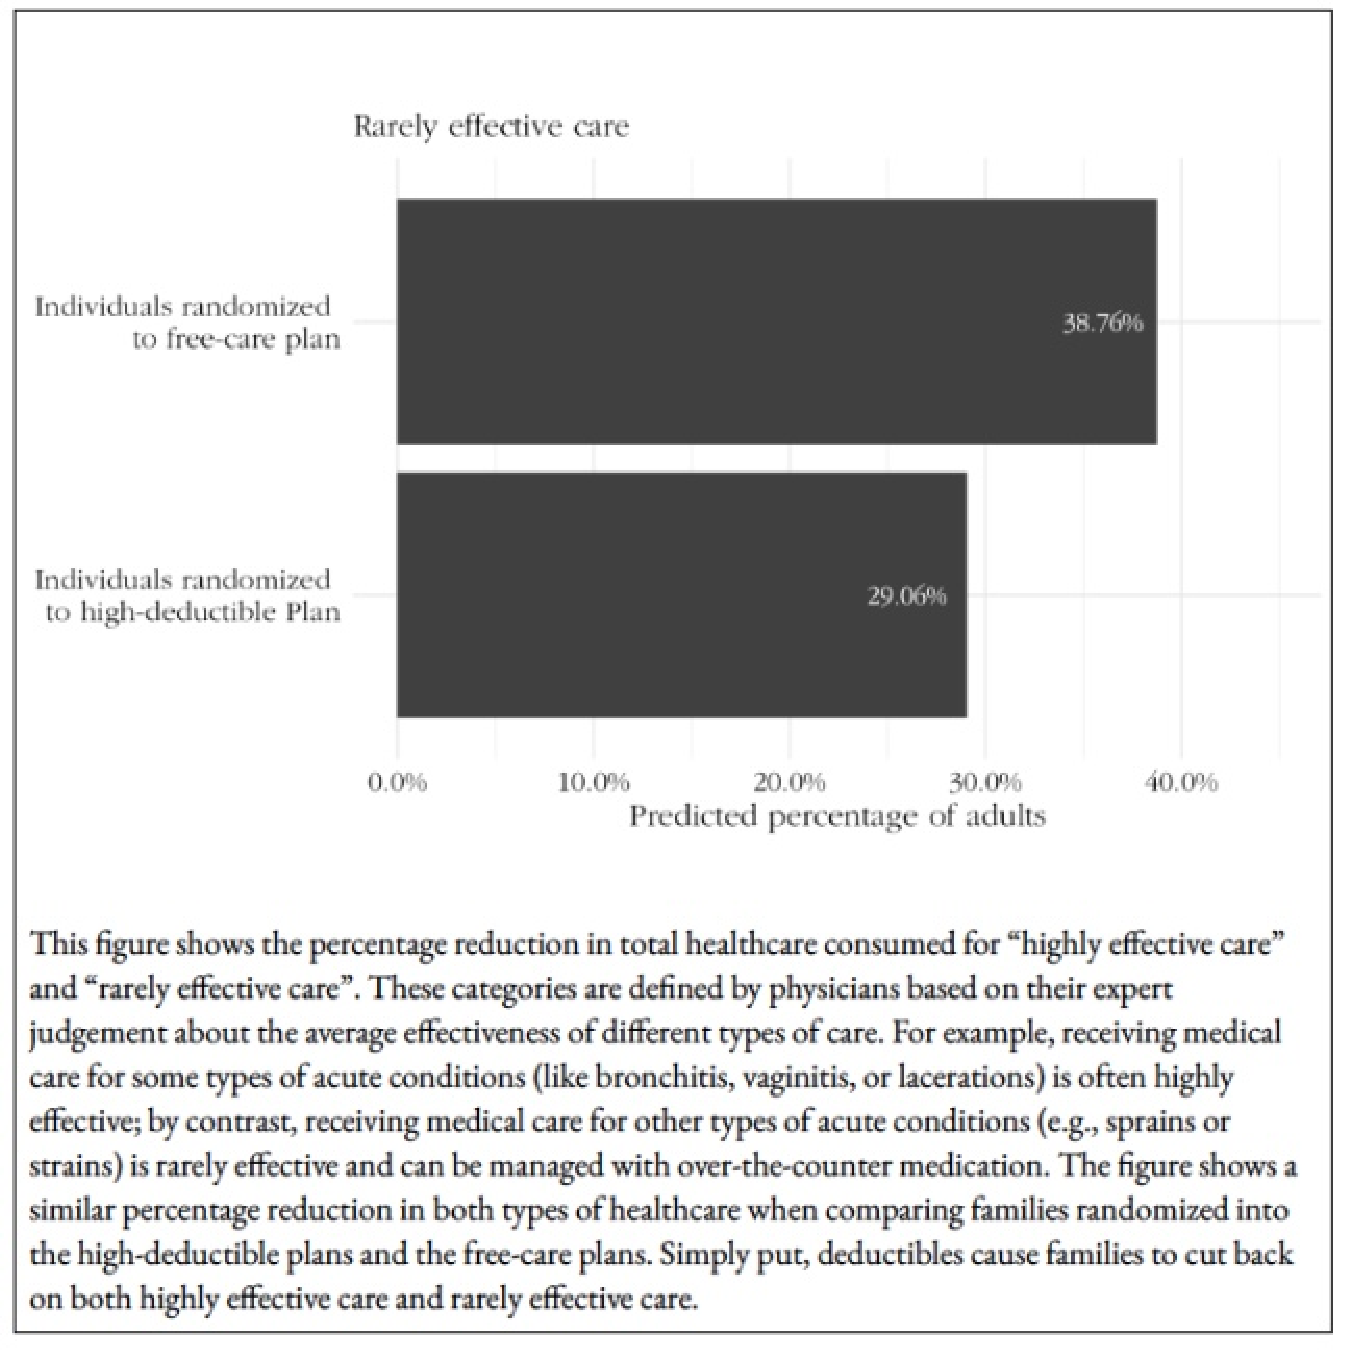
\includegraphics[width=0.45\textwidth]{input/RAND_rarelyeffectivecare.pdf}
    \end{center}
    \textcolor{white}{$\implies$ Which care is cut? Both ``rarely effective'' and ``effective'' care.}
    } \only<2>{
        \begin{center}
            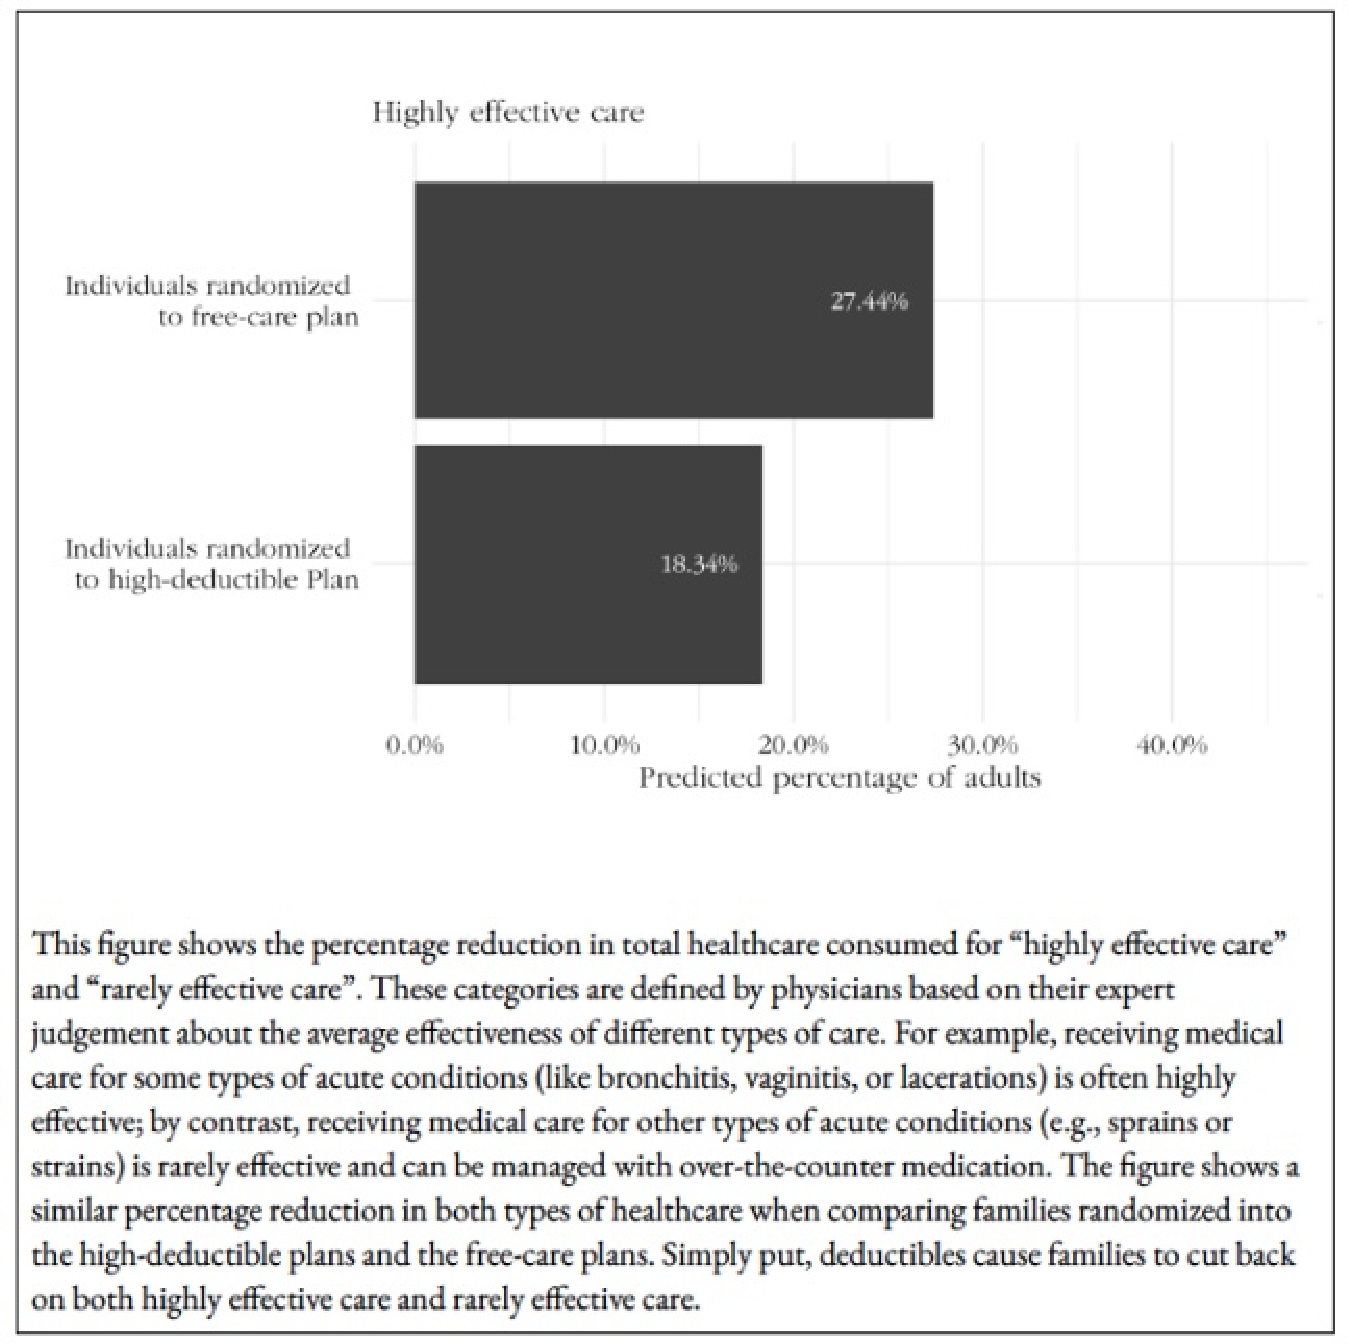
\includegraphics[width=0.45\textwidth]{input/RAND_effectivecare.pdf}
        \end{center}
        \textcolor{white}{$\implies$ Which care is cut? Both ``rarely effective'' and ``effective'' care.}
        }
    \only<3>{
        \begin{center}
            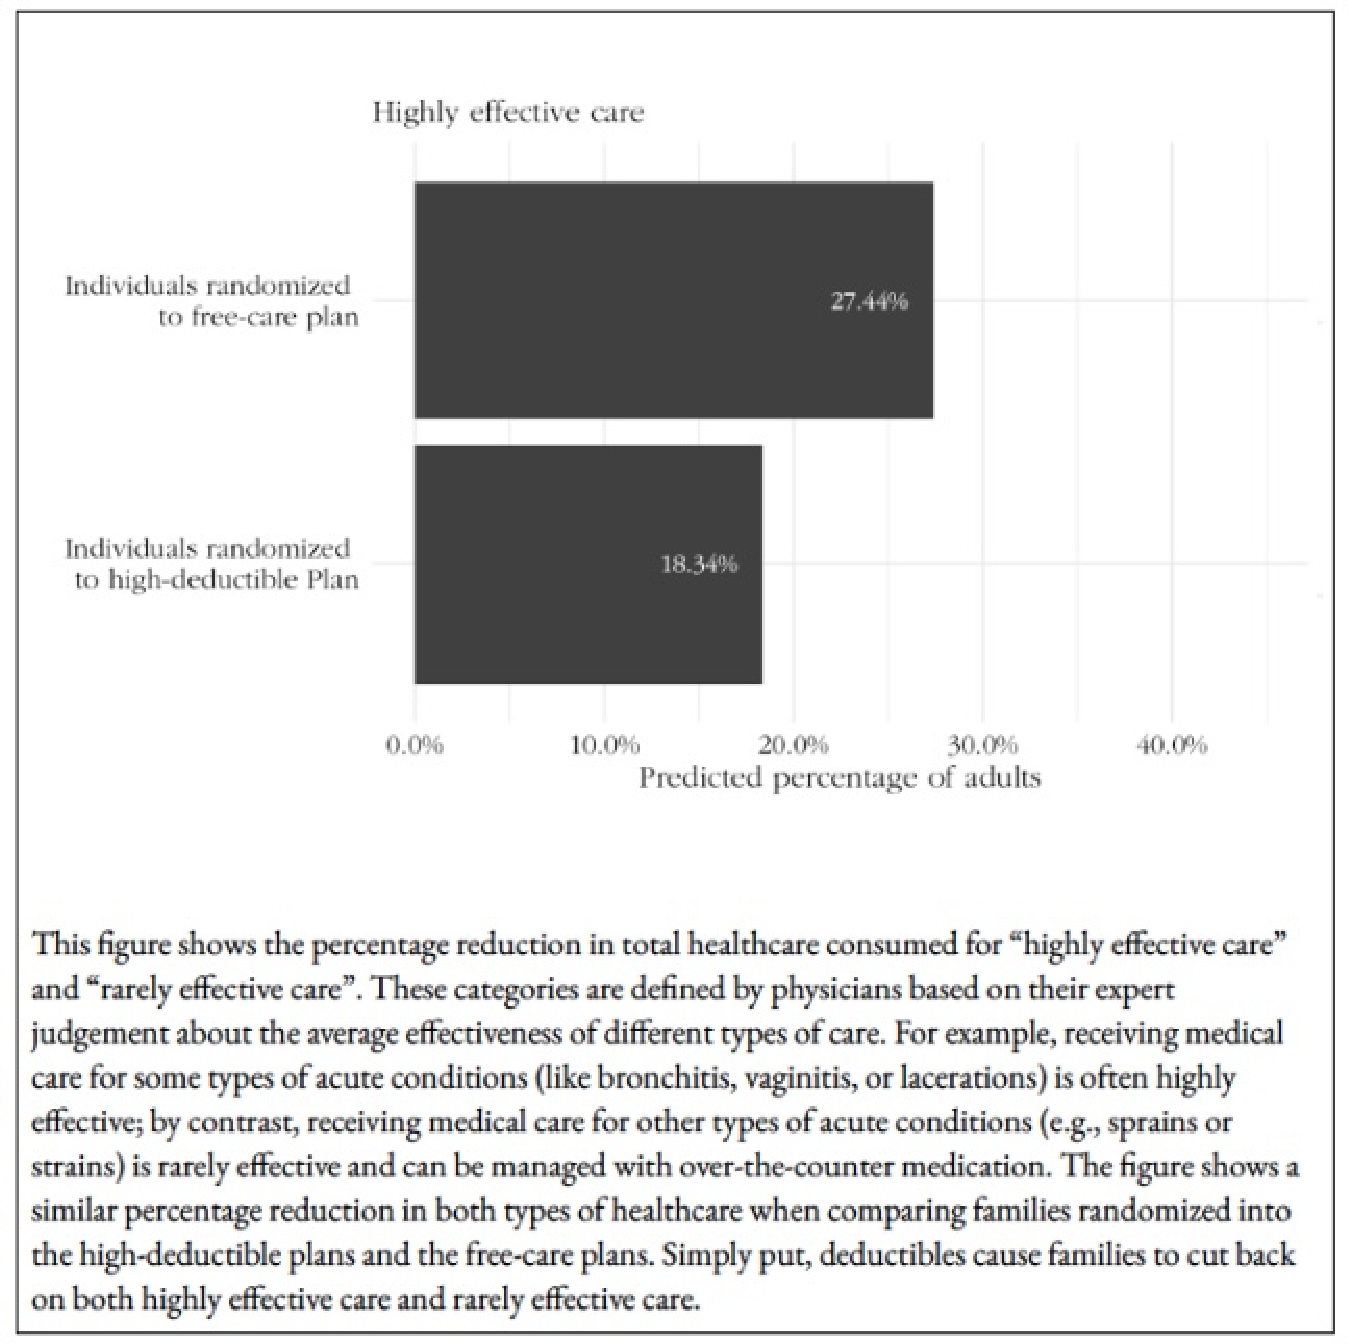
\includegraphics[width=0.45\textwidth]{input/RAND_effectivecare.pdf}
        \end{center}
        $\implies$ Which care is cut? Both ``rarely effective'' and ``effective'' care.
        }
\end{frame}
%---------------------------------------------------------------------
\begin{frame}{Impact on health?}

    \only<2>{
    \begin{center}
        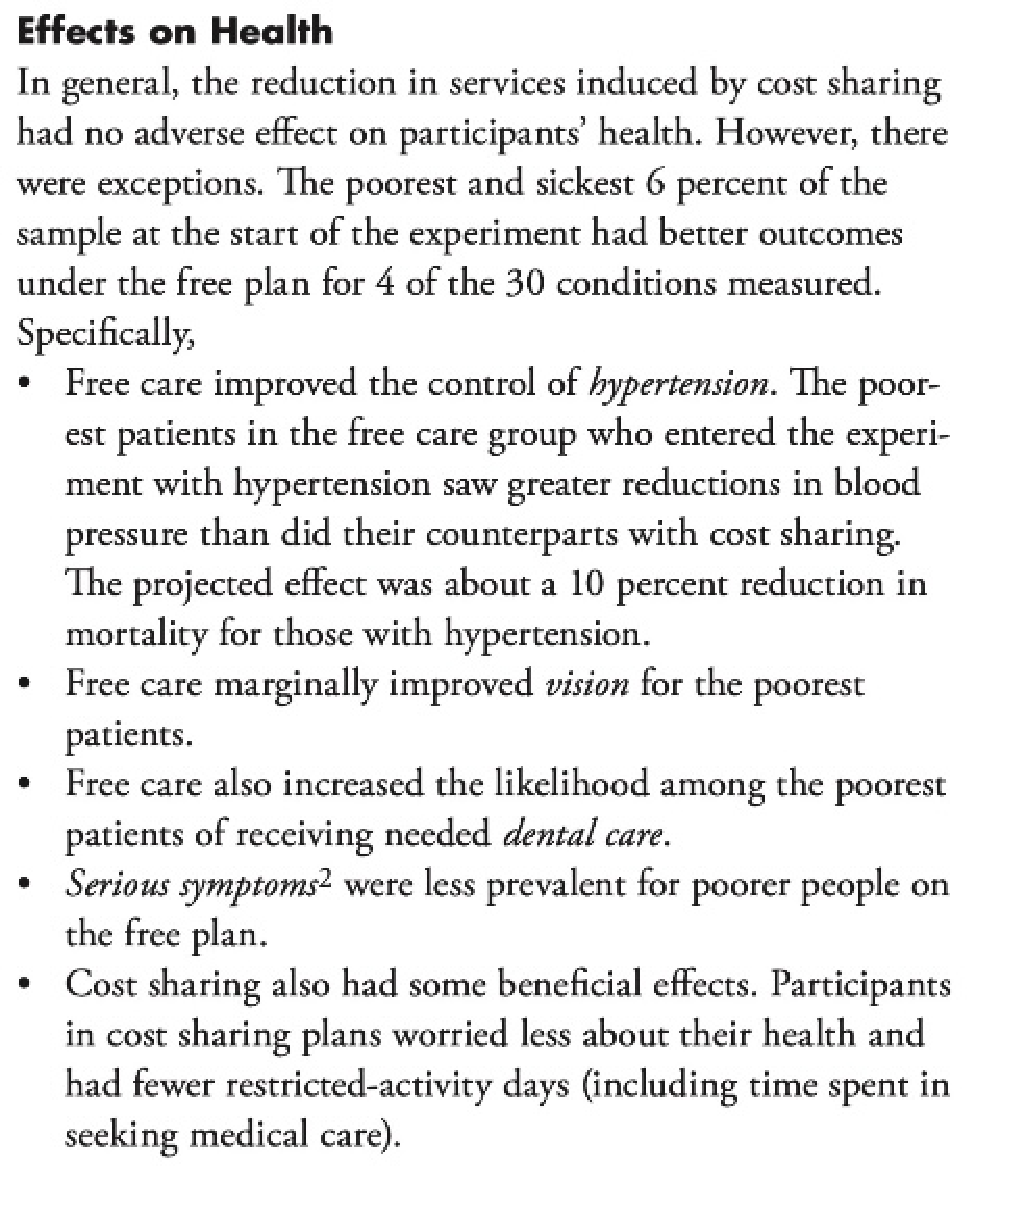
\includegraphics[width=0.4\textwidth]{input/RAND_effecthealth.pdf}
    \end{center}
    }

\end{frame}
%---------------------------------------------------------------------
\begin{frame}{The \newbold{RAND health insurance experiment}: conclusion}

    Main results:
    \begin{itemize}
        \item Healthcare demand slopes down
        \item Insurance increases the demand for healthcare
        \item Which care is cut: both ``effective'' and ``rarely effective'' care
        \item Impact on health? None on average but poor adults are hurt
    \end{itemize}
    \vspace{3mm}
  
        
    Legacy
        \begin{itemize}
            \item Largest and most expensive RCT in social science to date
            \item No impact on health: paved the way for cost-sharing (80s) and \textcolor{gray}{high-deductible} plans (2000s)
        \end{itemize}

\end{frame}
%---------------------------------------------------------------------
%---------------------------------------------------------------------
\begin{frame}{}
    \begin{center}
    \Large \textcolor{maroon}{Wraping up}
    \end{center}

\end{frame}
%---------------------------------------------------------------------
\begin{frame}{What we covered today}
    \begin{enumerate}
        \item \newbold{Microeconomics review}: budget constraint, preferences, demand
        \begin{itemize}
            \item \textit{Be comfortable with these concepts!}
        \end{itemize}
        \vspace{5mm}
    
        \item \newbold{Demand for healthcare}
        \begin{itemize}
            \item Is healthcare different than other goods? \newbold{No}
            \item The RAND health insurance experiment
        \end{itemize}
    \end{enumerate}
\end{frame}
%---------------------------------------------------------------------
\begin{frame}{To next class}
    \begin{itemize}
        \item \newbold{TO DO}
        \begin{enumerate}
            \item Review past material $\implies$ \textit{questions on it?}
        \end{enumerate}
        \vspace{5mm}

        \item Program for next class
        \begin{itemize}
            \item Demand for \textit{health}
        \end{itemize}
    \end{itemize}
\end{frame}
%---------------------------------------------------------------------
